% Options for packages loaded elsewhere
\PassOptionsToPackage{unicode}{hyperref}
\PassOptionsToPackage{hyphens}{url}
%
\documentclass[
]{article}
\usepackage{amsmath,amssymb}
\usepackage{iftex}
\ifPDFTeX
  \usepackage[T1]{fontenc}
  \usepackage[utf8]{inputenc}
  \usepackage{textcomp} % provide euro and other symbols
\else % if luatex or xetex
  \usepackage{unicode-math} % this also loads fontspec
  \defaultfontfeatures{Scale=MatchLowercase}
  \defaultfontfeatures[\rmfamily]{Ligatures=TeX,Scale=1}
\fi
\usepackage{lmodern}
\ifPDFTeX\else
  % xetex/luatex font selection
\fi
% Use upquote if available, for straight quotes in verbatim environments
\IfFileExists{upquote.sty}{\usepackage{upquote}}{}
\IfFileExists{microtype.sty}{% use microtype if available
  \usepackage[]{microtype}
  \UseMicrotypeSet[protrusion]{basicmath} % disable protrusion for tt fonts
}{}
\makeatletter
\@ifundefined{KOMAClassName}{% if non-KOMA class
  \IfFileExists{parskip.sty}{%
    \usepackage{parskip}
  }{% else
    \setlength{\parindent}{0pt}
    \setlength{\parskip}{6pt plus 2pt minus 1pt}}
}{% if KOMA class
  \KOMAoptions{parskip=half}}
\makeatother
\usepackage{xcolor}
\usepackage[margin=1in]{geometry}
\usepackage{color}
\usepackage{fancyvrb}
\newcommand{\VerbBar}{|}
\newcommand{\VERB}{\Verb[commandchars=\\\{\}]}
\DefineVerbatimEnvironment{Highlighting}{Verbatim}{commandchars=\\\{\}}
% Add ',fontsize=\small' for more characters per line
\usepackage{framed}
\definecolor{shadecolor}{RGB}{248,248,248}
\newenvironment{Shaded}{\begin{snugshade}}{\end{snugshade}}
\newcommand{\AlertTok}[1]{\textcolor[rgb]{0.94,0.16,0.16}{#1}}
\newcommand{\AnnotationTok}[1]{\textcolor[rgb]{0.56,0.35,0.01}{\textbf{\textit{#1}}}}
\newcommand{\AttributeTok}[1]{\textcolor[rgb]{0.13,0.29,0.53}{#1}}
\newcommand{\BaseNTok}[1]{\textcolor[rgb]{0.00,0.00,0.81}{#1}}
\newcommand{\BuiltInTok}[1]{#1}
\newcommand{\CharTok}[1]{\textcolor[rgb]{0.31,0.60,0.02}{#1}}
\newcommand{\CommentTok}[1]{\textcolor[rgb]{0.56,0.35,0.01}{\textit{#1}}}
\newcommand{\CommentVarTok}[1]{\textcolor[rgb]{0.56,0.35,0.01}{\textbf{\textit{#1}}}}
\newcommand{\ConstantTok}[1]{\textcolor[rgb]{0.56,0.35,0.01}{#1}}
\newcommand{\ControlFlowTok}[1]{\textcolor[rgb]{0.13,0.29,0.53}{\textbf{#1}}}
\newcommand{\DataTypeTok}[1]{\textcolor[rgb]{0.13,0.29,0.53}{#1}}
\newcommand{\DecValTok}[1]{\textcolor[rgb]{0.00,0.00,0.81}{#1}}
\newcommand{\DocumentationTok}[1]{\textcolor[rgb]{0.56,0.35,0.01}{\textbf{\textit{#1}}}}
\newcommand{\ErrorTok}[1]{\textcolor[rgb]{0.64,0.00,0.00}{\textbf{#1}}}
\newcommand{\ExtensionTok}[1]{#1}
\newcommand{\FloatTok}[1]{\textcolor[rgb]{0.00,0.00,0.81}{#1}}
\newcommand{\FunctionTok}[1]{\textcolor[rgb]{0.13,0.29,0.53}{\textbf{#1}}}
\newcommand{\ImportTok}[1]{#1}
\newcommand{\InformationTok}[1]{\textcolor[rgb]{0.56,0.35,0.01}{\textbf{\textit{#1}}}}
\newcommand{\KeywordTok}[1]{\textcolor[rgb]{0.13,0.29,0.53}{\textbf{#1}}}
\newcommand{\NormalTok}[1]{#1}
\newcommand{\OperatorTok}[1]{\textcolor[rgb]{0.81,0.36,0.00}{\textbf{#1}}}
\newcommand{\OtherTok}[1]{\textcolor[rgb]{0.56,0.35,0.01}{#1}}
\newcommand{\PreprocessorTok}[1]{\textcolor[rgb]{0.56,0.35,0.01}{\textit{#1}}}
\newcommand{\RegionMarkerTok}[1]{#1}
\newcommand{\SpecialCharTok}[1]{\textcolor[rgb]{0.81,0.36,0.00}{\textbf{#1}}}
\newcommand{\SpecialStringTok}[1]{\textcolor[rgb]{0.31,0.60,0.02}{#1}}
\newcommand{\StringTok}[1]{\textcolor[rgb]{0.31,0.60,0.02}{#1}}
\newcommand{\VariableTok}[1]{\textcolor[rgb]{0.00,0.00,0.00}{#1}}
\newcommand{\VerbatimStringTok}[1]{\textcolor[rgb]{0.31,0.60,0.02}{#1}}
\newcommand{\WarningTok}[1]{\textcolor[rgb]{0.56,0.35,0.01}{\textbf{\textit{#1}}}}
\usepackage{graphicx}
\makeatletter
\def\maxwidth{\ifdim\Gin@nat@width>\linewidth\linewidth\else\Gin@nat@width\fi}
\def\maxheight{\ifdim\Gin@nat@height>\textheight\textheight\else\Gin@nat@height\fi}
\makeatother
% Scale images if necessary, so that they will not overflow the page
% margins by default, and it is still possible to overwrite the defaults
% using explicit options in \includegraphics[width, height, ...]{}
\setkeys{Gin}{width=\maxwidth,height=\maxheight,keepaspectratio}
% Set default figure placement to htbp
\makeatletter
\def\fps@figure{htbp}
\makeatother
\setlength{\emergencystretch}{3em} % prevent overfull lines
\providecommand{\tightlist}{%
  \setlength{\itemsep}{0pt}\setlength{\parskip}{0pt}}
\setcounter{secnumdepth}{-\maxdimen} % remove section numbering
\ifLuaTeX
  \usepackage{selnolig}  % disable illegal ligatures
\fi
\IfFileExists{bookmark.sty}{\usepackage{bookmark}}{\usepackage{hyperref}}
\IfFileExists{xurl.sty}{\usepackage{xurl}}{} % add URL line breaks if available
\urlstyle{same}
\hypersetup{
  pdftitle={Submodule 1.3},
  pdfauthor={Plotting in R (ggplot)},
  hidelinks,
  pdfcreator={LaTeX via pandoc}}

\title{Submodule 1.3}
\author{Plotting in R (ggplot)}
\date{Spring 2024}

\begin{document}
\maketitle

Visualization often plays a major role in the research process, from
quality assurance, to data exploration, to the presentation of results.

The data visualization package \emph{ggplot2} makes it very easy and
straightforward to create a lot of different types of plots, from simple
to complex. In this module, we'll introduce ggplot syntax and briefly
survey some of the package's plotting capabilities.

A good ggplot cheat sheet can be found here:
\href{https://raw.githubusercontent.com/rstudio/cheatsheets/main/data-visualization.pdf}{ggplot
cheat sheet}

\hypertarget{load-script-for-submodule-1.3-plotting}{%
\subsection{Load script for submodule \#1.3:
Plotting}\label{load-script-for-submodule-1.3-plotting}}

\begin{enumerate}
\def\labelenumi{\arabic{enumi}.}
\item
  Click \href{module1_3.R}{here} to download the script, and save the
  script to your working directory (R Project folder).
\item
  Load the script into your RStudio Project. To do this, open your
  RStudio Project and click on the folder icon in the toolbar at the top
  and load your script.
\end{enumerate}

Let's get started with plotting in R!

\hypertarget{ggplot-basics}{%
\subsection{ggplot basics}\label{ggplot-basics}}

A typical workflow begins with initiating plotting with the
\textbf{\texttt{ggplot()}} function and specifying the data frame you
want to use to create your visualizations. We then often define the
``x'' argument (defining coordinates on an x axis) and (if applicable) a
``y'' argument (defining coordinates on a y axis). In ggplot these are
known as aesthetic mappings! That is because it is a way of conveying
information in the dataset graphically! Other ways of conveying
information graphically include point size, color, and symbol- all of
which are also referred to as aesthetic mappings (syntax:
\texttt{mapping=aes()}).

You can then add geometric objects (like points) to your plot, often
using functions beginning with \textbf{\texttt{geom\_}}, to represent
your data in the form of a boxplot (\textbf{\texttt{geom\_boxplot()}}),
scatterplot (\textbf{\texttt{geom\_point()}}), or a variety of other
types of plots. The \textbf{\texttt{aes()}} function can be called
within these ``geoms'' to specify which variables to display and how
these data should be displayed (which data should be used to represent
the bar height, or the x coordinate, or the point size, etc.).
\textbf{\texttt{aes()}} can also be used within the initial call to
\textbf{\texttt{ggplot()}}.

Here is an example of a simple \textbf{scatterplot} in ggplot:

\begin{Shaded}
\begin{Highlighting}[]
\CommentTok{\# scatterplots {-}{-}{-}{-}{-}{-}{-}{-}{-}{-}{-}{-}{-}{-}{-}{-}{-}{-}{-}{-}{-}{-}{-}{-}{-}{-}{-}{-}}

\FunctionTok{ggplot}\NormalTok{(trees, }\FunctionTok{aes}\NormalTok{(}\AttributeTok{x=}\NormalTok{Girth,}\AttributeTok{y=}\NormalTok{Volume)) }\SpecialCharTok{+}
  \FunctionTok{geom\_point}\NormalTok{()}
\end{Highlighting}
\end{Shaded}

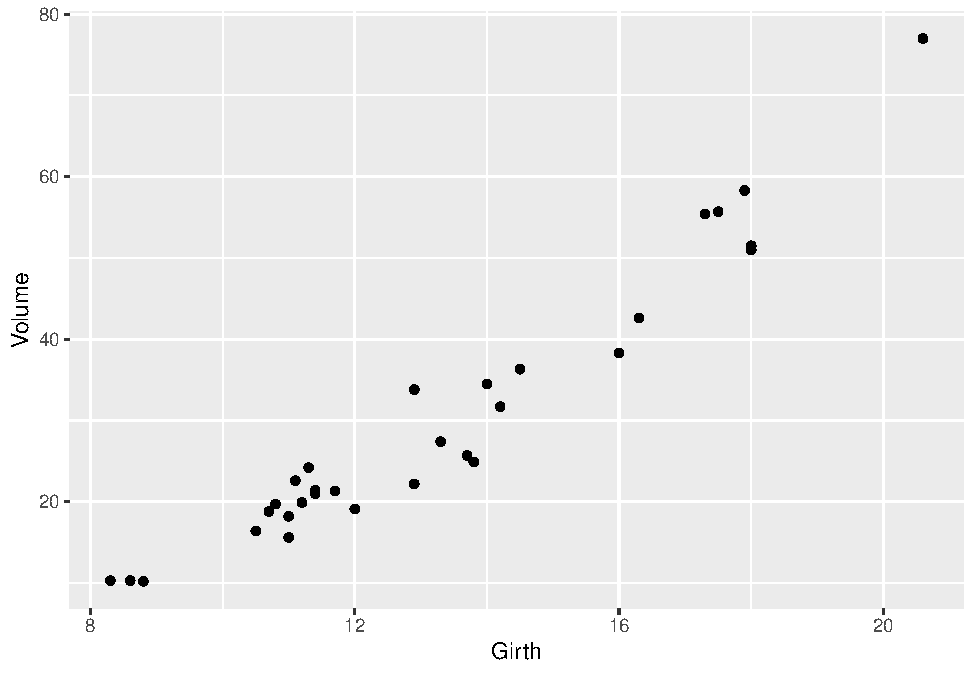
\includegraphics{module1_3_files/figure-latex/unnamed-chunk-7-1.pdf}

We'll start with the `trees' dataset, which is built into R. It
describes the girth, height, and volume of 31 felled black cherry trees.

\begin{Shaded}
\begin{Highlighting}[]
\CommentTok{\# ASIDE: explore the built{-}in \textquotesingle{}trees\textquotesingle{} dataset}

\CommentTok{\# ?trees      \# description of built in dataset  (uncomment to run)}

\FunctionTok{dim}\NormalTok{(trees)   }\CommentTok{\# Show the dimension of the trees dataframe                                              }
\end{Highlighting}
\end{Shaded}

\begin{verbatim}
## [1] 31  3
\end{verbatim}

\begin{Shaded}
\begin{Highlighting}[]
\FunctionTok{str}\NormalTok{(trees)   }\CommentTok{\# Show the structure of the trees dataframe}
\end{Highlighting}
\end{Shaded}

\begin{verbatim}
## 'data.frame':    31 obs. of  3 variables:
##  $ Girth : num  8.3 8.6 8.8 10.5 10.7 10.8 11 11 11.1 11.2 ...
##  $ Height: num  70 65 63 72 81 83 66 75 80 75 ...
##  $ Volume: num  10.3 10.3 10.2 16.4 18.8 19.7 15.6 18.2 22.6 19.9 ...
\end{verbatim}

\begin{Shaded}
\begin{Highlighting}[]
\FunctionTok{head}\NormalTok{(trees)   }\CommentTok{\# Show the first few observations of the trees dataframe}

\FunctionTok{summary}\NormalTok{(trees)  }\CommentTok{\# Summary stats for each column}
\end{Highlighting}
\end{Shaded}

\begin{verbatim}
##      Girth           Height       Volume     
##  Min.   : 8.30   Min.   :63   Min.   :10.20  
##  1st Qu.:11.05   1st Qu.:72   1st Qu.:19.40  
##  Median :12.90   Median :76   Median :24.20  
##  Mean   :13.25   Mean   :76   Mean   :30.17  
##  3rd Qu.:15.25   3rd Qu.:80   3rd Qu.:37.30  
##  Max.   :20.60   Max.   :87   Max.   :77.00
\end{verbatim}

And some more fancy and informative scatterplots

\begin{Shaded}
\begin{Highlighting}[]
    \CommentTok{\# try representing tree height using the color aesthetic}
\FunctionTok{ggplot}\NormalTok{(trees, }\FunctionTok{aes}\NormalTok{(}\AttributeTok{x=}\NormalTok{Girth,}\AttributeTok{y=}\NormalTok{Volume)) }\SpecialCharTok{+}
  \FunctionTok{geom\_point}\NormalTok{(}\FunctionTok{aes}\NormalTok{(}\AttributeTok{col=}\NormalTok{Height))}
\end{Highlighting}
\end{Shaded}

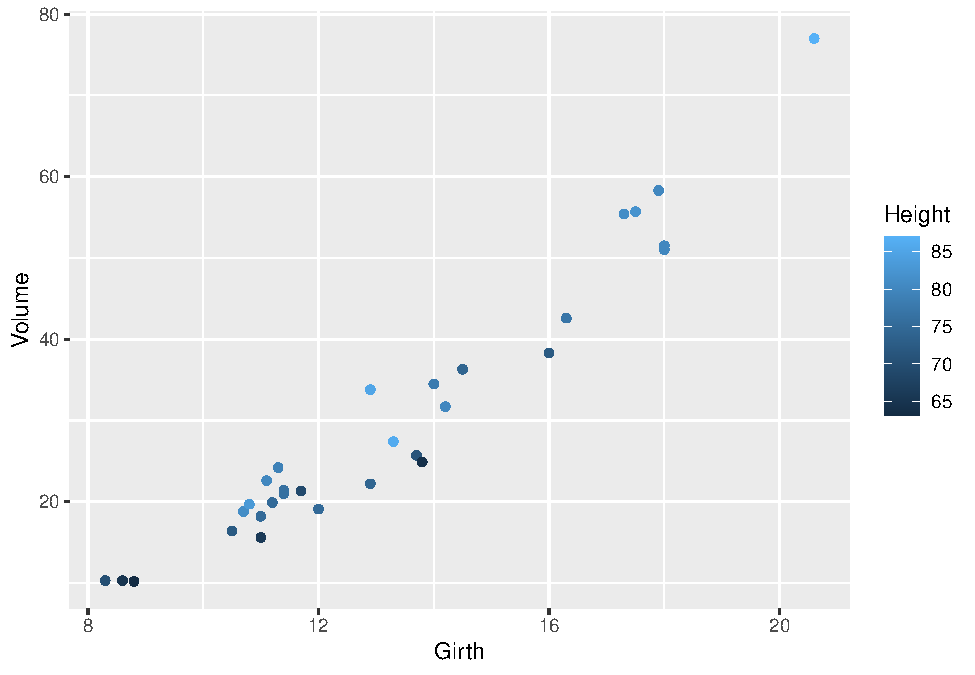
\includegraphics{module1_3_files/figure-latex/unnamed-chunk-9-1.pdf}

\begin{Shaded}
\begin{Highlighting}[]
    \CommentTok{\# try representing tree height using the size aesthetic}
\FunctionTok{ggplot}\NormalTok{(trees, }\FunctionTok{aes}\NormalTok{(}\AttributeTok{x=}\NormalTok{Girth,}\AttributeTok{y=}\NormalTok{Volume)) }\SpecialCharTok{+}
  \FunctionTok{geom\_point}\NormalTok{(}\FunctionTok{aes}\NormalTok{(}\AttributeTok{size=}\NormalTok{Height))}
\end{Highlighting}
\end{Shaded}

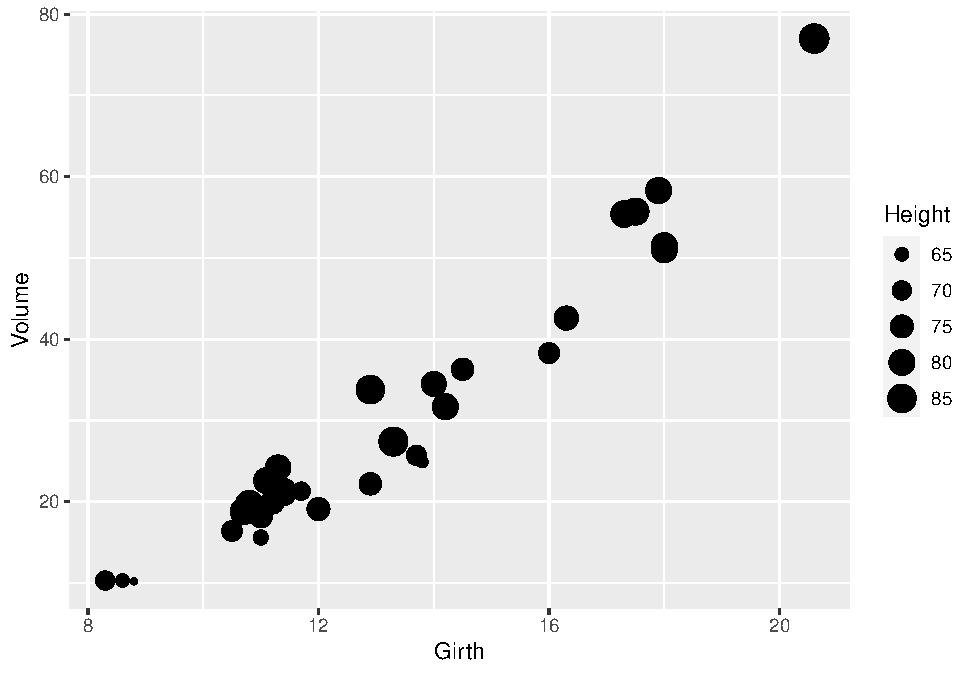
\includegraphics{module1_3_files/figure-latex/unnamed-chunk-9-2.pdf}

\begin{Shaded}
\begin{Highlighting}[]
   \CommentTok{\# try adding a regression line}
\FunctionTok{ggplot}\NormalTok{(trees, }\FunctionTok{aes}\NormalTok{(}\AttributeTok{x=}\NormalTok{Girth,}\AttributeTok{y=}\NormalTok{Volume)) }\SpecialCharTok{+}
  \FunctionTok{geom\_point}\NormalTok{() }\SpecialCharTok{+}
  \FunctionTok{geom\_smooth}\NormalTok{(}\AttributeTok{method=}\StringTok{"lm"}\NormalTok{)}
\end{Highlighting}
\end{Shaded}

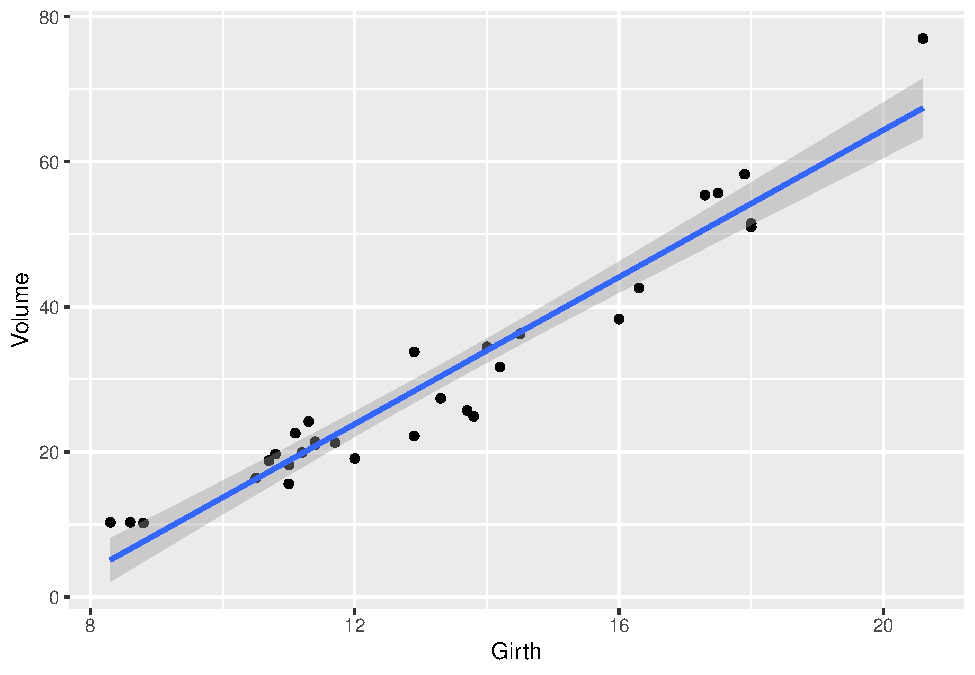
\includegraphics{module1_3_files/figure-latex/unnamed-chunk-9-3.pdf}

\hypertarget{change-plot-type}{%
\subsubsection{Change Plot Type}\label{change-plot-type}}

Because we're exploring different ways of plotting, it is useful to
include multiple plots in the same image.

We can do this using the \texttt{plot\_grid()} function in the cowplot
package (commonly used extensions to ggplot). Here we explore different
ways of graphically representing the relationship between tree girth and
volume.

\begin{Shaded}
\begin{Highlighting}[]
\CommentTok{\# Explore different "geoms" or plot types }

\NormalTok{plot1 }\OtherTok{\textless{}{-}} \FunctionTok{ggplot}\NormalTok{(trees,}\FunctionTok{aes}\NormalTok{(Girth,Volume)) }\SpecialCharTok{+}    \CommentTok{\# plot the relationship as a line}
  \FunctionTok{geom\_line}\NormalTok{()}
\NormalTok{plot2 }\OtherTok{\textless{}{-}} \FunctionTok{ggplot}\NormalTok{(trees,}\FunctionTok{aes}\NormalTok{(Girth,Volume)) }\SpecialCharTok{+}    \CommentTok{\# plot a smoothed "spline" fit of the relationship}
  \FunctionTok{geom\_smooth}\NormalTok{()}
\NormalTok{plot3 }\OtherTok{\textless{}{-}} \FunctionTok{ggplot}\NormalTok{(trees,}\FunctionTok{aes}\NormalTok{(Girth,Volume)) }\SpecialCharTok{+}    \CommentTok{\# plot scatterplot}
  \FunctionTok{geom\_point}\NormalTok{() }
\NormalTok{plot4 }\OtherTok{\textless{}{-}} \FunctionTok{ggplot}\NormalTok{(trees,}\FunctionTok{aes}\NormalTok{(Girth,Volume)) }\SpecialCharTok{+}    \CommentTok{\# plot scatterplot with smoothed regression line}
  \FunctionTok{geom\_point}\NormalTok{() }\SpecialCharTok{+} 
  \FunctionTok{geom\_smooth}\NormalTok{()}
\FunctionTok{plot\_grid}\NormalTok{(plot1,plot2,plot3,plot4,}\AttributeTok{labels=}\StringTok{"auto"}\NormalTok{)}
\end{Highlighting}
\end{Shaded}

\hypertarget{change-symbols-colors-and-point-sizes}{%
\subsubsection{Change symbols, colors and point
sizes}\label{change-symbols-colors-and-point-sizes}}

Point shape is specified using the \texttt{shape=} option.

Color is specified using the \texttt{color=} option.

Size is specified using the \texttt{size=} option.

If you want convey information in your data via the color, symbol, or
point size, you include it as an aesthetic mapping- and link it to one
of the columns in your data.

If you just want to color all the points the same way, or use the same
symbol for everything, specify this outside of the aesthetic mapping.

To illustrate this, let's use the built in \texttt{iris} dataset, which
gives the sepal length/width and petal length/width (in cm), for 50
flowers from each of 3 iris species.

\begin{Shaded}
\begin{Highlighting}[]
\CommentTok{\# Explore different aesthetic mappings }

\NormalTok{plot1 }\OtherTok{\textless{}{-}} \FunctionTok{ggplot}\NormalTok{(iris,}\FunctionTok{aes}\NormalTok{(Sepal.Length,Petal.Length)) }\SpecialCharTok{+}    \CommentTok{\# shape represents species}
  \FunctionTok{geom\_point}\NormalTok{(}\FunctionTok{aes}\NormalTok{(}\AttributeTok{shape=}\NormalTok{Species))}
\NormalTok{plot2 }\OtherTok{\textless{}{-}} \FunctionTok{ggplot}\NormalTok{(iris,}\FunctionTok{aes}\NormalTok{(Sepal.Length,Petal.Length)) }\SpecialCharTok{+}       \CommentTok{\# shape is same for everything!}
  \FunctionTok{geom\_point}\NormalTok{(}\AttributeTok{shape=}\DecValTok{2}\NormalTok{)}
\NormalTok{plot3 }\OtherTok{\textless{}{-}} \FunctionTok{ggplot}\NormalTok{(iris,}\FunctionTok{aes}\NormalTok{(Sepal.Length,Petal.Length)) }\SpecialCharTok{+}    \CommentTok{\# color represents species}
  \FunctionTok{geom\_point}\NormalTok{(}\FunctionTok{aes}\NormalTok{(}\AttributeTok{color=}\NormalTok{Species)) }
\NormalTok{plot4 }\OtherTok{\textless{}{-}} \FunctionTok{ggplot}\NormalTok{(iris,}\FunctionTok{aes}\NormalTok{(Sepal.Length,Petal.Length)) }\SpecialCharTok{+}    \CommentTok{\# color is same across the board}
  \FunctionTok{geom\_point}\NormalTok{(}\AttributeTok{col=}\StringTok{"purple"}\NormalTok{)  }
\NormalTok{plot5 }\OtherTok{\textless{}{-}} \FunctionTok{ggplot}\NormalTok{(iris,}\FunctionTok{aes}\NormalTok{(Sepal.Length,Petal.Length)) }\SpecialCharTok{+}    \CommentTok{\# size represents species}
  \FunctionTok{geom\_point}\NormalTok{(}\FunctionTok{aes}\NormalTok{(}\AttributeTok{size=}\NormalTok{Species)) }
\NormalTok{plot6 }\OtherTok{\textless{}{-}} \FunctionTok{ggplot}\NormalTok{(iris,}\FunctionTok{aes}\NormalTok{(Sepal.Length,Petal.Length)) }\SpecialCharTok{+}    \CommentTok{\# size is same across the board}
  \FunctionTok{geom\_point}\NormalTok{(}\AttributeTok{size=}\DecValTok{2}\NormalTok{) }
\FunctionTok{plot\_grid}\NormalTok{(plot1,plot2,plot3,plot4,plot5,plot6,}\AttributeTok{ncol=}\DecValTok{2}\NormalTok{)}
\end{Highlighting}
\end{Shaded}

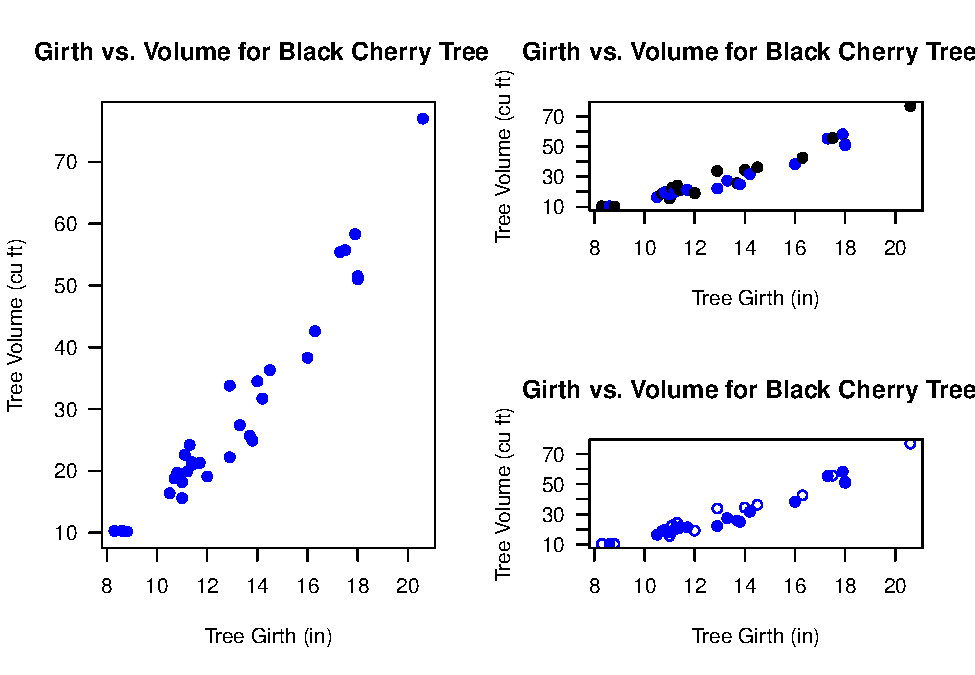
\includegraphics{module1_3_files/figure-latex/unnamed-chunk-11-1.pdf}

Here is a graphic illustrating the main plot symbols you can reference
using \texttt{shape=}:

\includegraphics{points.png} Colors are a bit more intuitive, but here's
a \href{http://www.stat.columbia.edu/~tzheng/files/Rcolor.pdf}{link to a
chart of R colors})

\hypertarget{themes}{%
\subsubsection{Themes}\label{themes}}

You can see that the default plot includes a gray background with white
gridlines. This makes all of the elements on this plot easy to see, but
as you start adjusting colors and identifying your personal preferences,
you'll probably want to customize this -- ggplot has a ton of options
for doing so. Here's a few examples of ggplot \textbf{themes}:

\begin{Shaded}
\begin{Highlighting}[]
\CommentTok{\# explore themes }

\NormalTok{plot1 }\OtherTok{\textless{}{-}} \FunctionTok{ggplot}\NormalTok{(iris,}\FunctionTok{aes}\NormalTok{(Sepal.Length,Petal.Length)) }\SpecialCharTok{+}    \CommentTok{\# color represents species}
  \FunctionTok{geom\_point}\NormalTok{(}\FunctionTok{aes}\NormalTok{(}\AttributeTok{color=}\NormalTok{Species)) }\SpecialCharTok{+}
  \FunctionTok{theme\_bw}\NormalTok{()}
\NormalTok{plot2 }\OtherTok{\textless{}{-}} \FunctionTok{ggplot}\NormalTok{(iris,}\FunctionTok{aes}\NormalTok{(Sepal.Length,Petal.Length)) }\SpecialCharTok{+}    \CommentTok{\# color represents species}
  \FunctionTok{geom\_point}\NormalTok{(}\FunctionTok{aes}\NormalTok{(}\AttributeTok{color=}\NormalTok{Species)) }\SpecialCharTok{+}
  \FunctionTok{theme\_classic}\NormalTok{()}
\NormalTok{plot3 }\OtherTok{\textless{}{-}} \FunctionTok{ggplot}\NormalTok{(iris,}\FunctionTok{aes}\NormalTok{(Sepal.Length,Petal.Length)) }\SpecialCharTok{+}    \CommentTok{\# color represents species}
  \FunctionTok{geom\_point}\NormalTok{(}\FunctionTok{aes}\NormalTok{(}\AttributeTok{color=}\NormalTok{Species)) }\SpecialCharTok{+}
  \FunctionTok{theme\_minimal}\NormalTok{()}
\NormalTok{plot4 }\OtherTok{\textless{}{-}} \FunctionTok{ggplot}\NormalTok{(iris,}\FunctionTok{aes}\NormalTok{(Sepal.Length,Petal.Length)) }\SpecialCharTok{+}    \CommentTok{\# color represents species}
  \FunctionTok{geom\_point}\NormalTok{(}\FunctionTok{aes}\NormalTok{(}\AttributeTok{color=}\NormalTok{Species)) }\SpecialCharTok{+}
  \FunctionTok{theme\_minimal\_grid}\NormalTok{(}\AttributeTok{font\_size =} \DecValTok{11}\NormalTok{)}

\FunctionTok{plot\_grid}\NormalTok{(plot1,plot2,plot3,plot4,}\AttributeTok{labels =} \StringTok{"AUTO"}\NormalTok{)}
\end{Highlighting}
\end{Shaded}

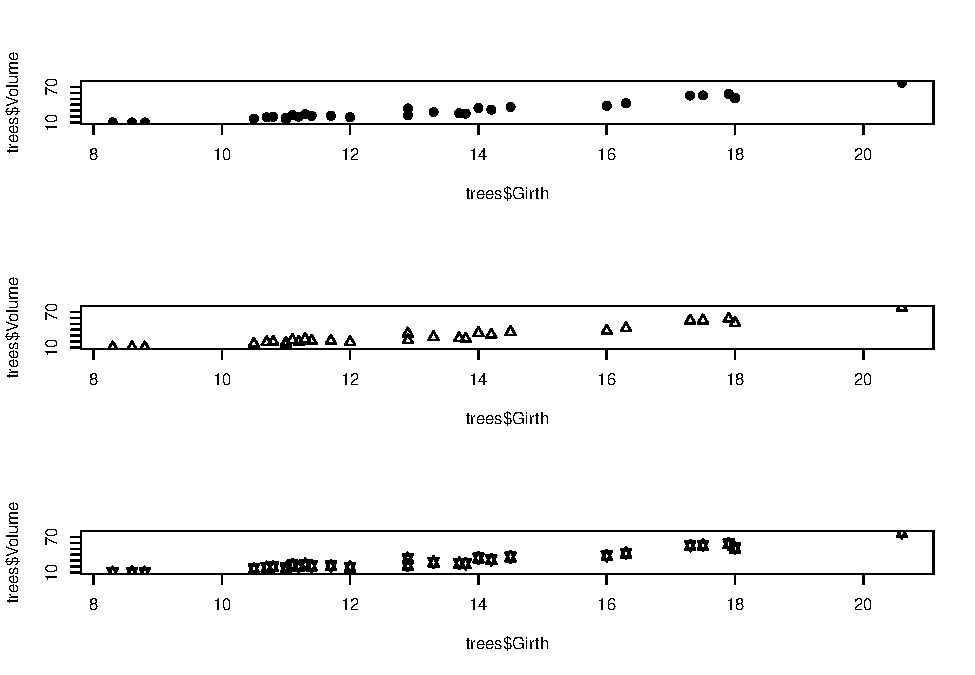
\includegraphics{module1_3_files/figure-latex/unnamed-chunk-12-1.pdf}

\begin{Shaded}
\begin{Highlighting}[]
\CommentTok{\# note: many other themes are available in ggplot, cowplot and other related packages}
\end{Highlighting}
\end{Shaded}

\hypertarget{changing-title-and-axis-labels}{%
\subsubsection{Changing title and axis
labels}\label{changing-title-and-axis-labels}}

We can also add titles, axis labels, and other options to make the plots
look prettier.

\begin{Shaded}
\begin{Highlighting}[]
\CommentTok{\# add additional plot elements: title, axis limis, axis labels }

\NormalTok{plot1 }\OtherTok{\textless{}{-}} \FunctionTok{ggplot}\NormalTok{(iris,}\FunctionTok{aes}\NormalTok{(Sepal.Length,Petal.Length)) }\SpecialCharTok{+}    \CommentTok{\# color represents species}
  \FunctionTok{geom\_point}\NormalTok{(}\FunctionTok{aes}\NormalTok{(}\AttributeTok{color=}\NormalTok{Species)) }\SpecialCharTok{+} 
  \FunctionTok{labs}\NormalTok{(}\AttributeTok{x=}\StringTok{"Sepal Length (cm)"}\NormalTok{)}

\NormalTok{plot2 }\OtherTok{\textless{}{-}} \FunctionTok{ggplot}\NormalTok{(iris,}\FunctionTok{aes}\NormalTok{(Sepal.Length,Petal.Length)) }\SpecialCharTok{+}    \CommentTok{\# color represents species}
  \FunctionTok{geom\_point}\NormalTok{(}\FunctionTok{aes}\NormalTok{(}\AttributeTok{color=}\NormalTok{Species)) }\SpecialCharTok{+} 
  \FunctionTok{labs}\NormalTok{(}\AttributeTok{x=}\StringTok{"Sepal Length (cm)"}\NormalTok{,}\AttributeTok{y=}\StringTok{"Petal Length (cm)"}\NormalTok{,}\AttributeTok{color=}\StringTok{"Iris sp."}\NormalTok{)}

\NormalTok{plot3 }\OtherTok{\textless{}{-}} \FunctionTok{ggplot}\NormalTok{(iris,}\FunctionTok{aes}\NormalTok{(Sepal.Length,Petal.Length)) }\SpecialCharTok{+}    \CommentTok{\# color represents species}
  \FunctionTok{geom\_point}\NormalTok{(}\FunctionTok{aes}\NormalTok{(}\AttributeTok{color=}\NormalTok{Species)) }\SpecialCharTok{+} 
  \FunctionTok{labs}\NormalTok{(}\AttributeTok{x=}\StringTok{"Sepal Length (cm)"}\NormalTok{,}\AttributeTok{y=}\StringTok{"Petal Length (cm)"}\NormalTok{,}\AttributeTok{color=}\StringTok{"Iris sp."}\NormalTok{,}
       \AttributeTok{title=}\StringTok{"Fisher\textquotesingle{}s Iris Data"}\NormalTok{,}\AttributeTok{subtitle =} \StringTok{"practice with ggplot"}\NormalTok{)}

\NormalTok{plot4 }\OtherTok{\textless{}{-}} \FunctionTok{ggplot}\NormalTok{(iris,}\FunctionTok{aes}\NormalTok{(Sepal.Length,Petal.Length)) }\SpecialCharTok{+}    \CommentTok{\# color represents species}
  \FunctionTok{geom\_point}\NormalTok{(}\FunctionTok{aes}\NormalTok{(}\AttributeTok{color=}\NormalTok{Species)) }\SpecialCharTok{+} 
  \FunctionTok{coord\_cartesian}\NormalTok{(}\AttributeTok{xlim=}\FunctionTok{c}\NormalTok{(}\DecValTok{0}\NormalTok{,}\DecValTok{10}\NormalTok{),}\AttributeTok{ylim=}\FunctionTok{c}\NormalTok{(}\DecValTok{0}\NormalTok{,}\DecValTok{10}\NormalTok{)) }\SpecialCharTok{+}
  \FunctionTok{labs}\NormalTok{(}\AttributeTok{x=}\StringTok{"Sepal Length (cm)"}\NormalTok{,}\AttributeTok{y=}\StringTok{"Petal Length (cm)"}\NormalTok{,}\AttributeTok{color=}\StringTok{"Iris sp."}\NormalTok{,}
       \AttributeTok{title=}\StringTok{"Fisher\textquotesingle{}s Iris Data"}\NormalTok{,}\AttributeTok{subtitle =} \StringTok{"practice with ggplot"}\NormalTok{)}

\FunctionTok{plot\_grid}\NormalTok{(plot1,plot2,plot3,plot4,}\AttributeTok{labels =} \StringTok{"AUTO"}\NormalTok{)}
\end{Highlighting}
\end{Shaded}

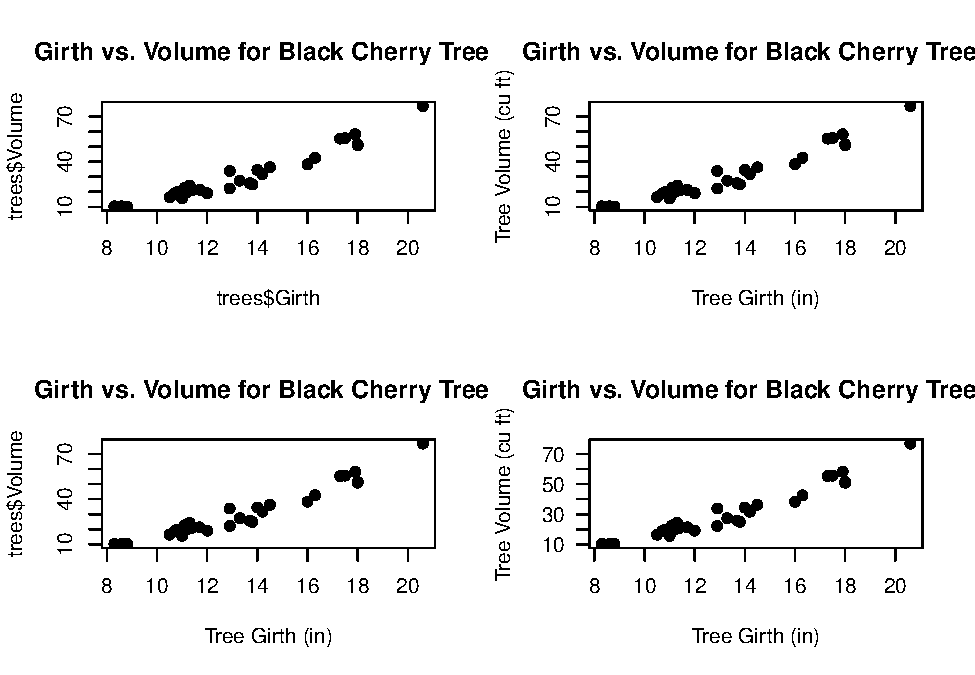
\includegraphics{module1_3_files/figure-latex/unnamed-chunk-13-1.pdf}

\hypertarget{bar-plots-and-box-whisker-plots}{%
\subsection{Bar Plots and box-whisker
plots}\label{bar-plots-and-box-whisker-plots}}

\begin{Shaded}
\begin{Highlighting}[]
\CommentTok{\# bar plots, box{-}whisker plots, violin plots  {-}{-}{-}{-}{-}{-}{-}{-}{-}{-}{-}{-}{-}{-}{-}{-}{-}{-}{-}{-}{-}{-}{-}}

\NormalTok{plot1 }\OtherTok{\textless{}{-}} \FunctionTok{ggplot}\NormalTok{(iris,}\FunctionTok{aes}\NormalTok{(}\AttributeTok{x=}\NormalTok{Species,}\AttributeTok{y=}\NormalTok{Sepal.Length)) }\SpecialCharTok{+}    \CommentTok{\# more informative box{-}whisker plot}
  \FunctionTok{geom\_boxplot}\NormalTok{() }
  
\NormalTok{plot2 }\OtherTok{\textless{}{-}} \FunctionTok{ggplot}\NormalTok{(iris,}\FunctionTok{aes}\NormalTok{(}\AttributeTok{x=}\NormalTok{Species,}\AttributeTok{y=}\NormalTok{Sepal.Length)) }\SpecialCharTok{+}    \CommentTok{\# more informative box{-}whisker plot +}
  \FunctionTok{geom\_violin}\NormalTok{() }

\CommentTok{\# bar plot}
\NormalTok{bar.heights }\OtherTok{\textless{}{-}}\NormalTok{ iris }\SpecialCharTok{\%\textgreater{}\%} 
  \FunctionTok{group\_by}\NormalTok{(Species) }\SpecialCharTok{\%\textgreater{}\%} 
  \FunctionTok{summarize}\NormalTok{(}\AttributeTok{meanSL =} \FunctionTok{mean}\NormalTok{(Sepal.Length))}

\NormalTok{plot3 }\OtherTok{\textless{}{-}} \FunctionTok{ggplot}\NormalTok{(bar.heights, }\FunctionTok{aes}\NormalTok{(Species,meanSL)) }\SpecialCharTok{+}
  \FunctionTok{geom\_col}\NormalTok{()}


\NormalTok{plot4 }\OtherTok{\textless{}{-}} \FunctionTok{ggplot}\NormalTok{(bar.heights, }\FunctionTok{aes}\NormalTok{(Species,meanSL)) }\SpecialCharTok{+}
  \FunctionTok{geom\_col}\NormalTok{(}\FunctionTok{aes}\NormalTok{(}\AttributeTok{fill=}\NormalTok{Species)) }\SpecialCharTok{+}
  \FunctionTok{theme\_classic}\NormalTok{() }\SpecialCharTok{+}
  \FunctionTok{scale\_fill\_manual}\NormalTok{(}\AttributeTok{values=}\FunctionTok{c}\NormalTok{(}\StringTok{"gray"}\NormalTok{,}\StringTok{"red"}\NormalTok{,}\StringTok{"brown"}\NormalTok{))}
  
\FunctionTok{plot\_grid}\NormalTok{(plot1,plot2,plot3,plot4,}\AttributeTok{labels =} \StringTok{"AUTO"}\NormalTok{)}
\end{Highlighting}
\end{Shaded}

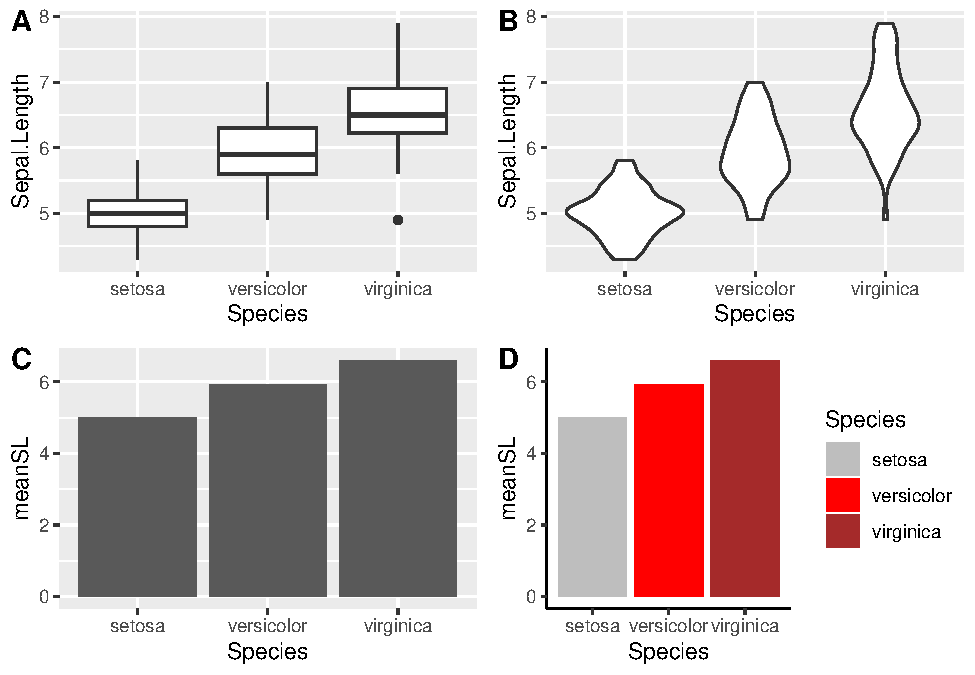
\includegraphics{module1_3_files/figure-latex/unnamed-chunk-14-1.pdf}

But what if we want to have some error bars?

\begin{Shaded}
\begin{Highlighting}[]
\CommentTok{\# Bar plot with error bars}

\NormalTok{bar.heights }\OtherTok{\textless{}{-}}\NormalTok{ iris }\SpecialCharTok{\%\textgreater{}\%} 
  \FunctionTok{group\_by}\NormalTok{(Species) }\SpecialCharTok{\%\textgreater{}\%} 
  \FunctionTok{summarize}\NormalTok{(}\AttributeTok{meanSL =} \FunctionTok{mean}\NormalTok{(Sepal.Length),}
            \AttributeTok{n =} \FunctionTok{n}\NormalTok{(),}
            \AttributeTok{sdSL =} \FunctionTok{sd}\NormalTok{(Sepal.Length),}
            \AttributeTok{se =}\NormalTok{ sdSL}\SpecialCharTok{/}\FunctionTok{sqrt}\NormalTok{(n))}
  
\FunctionTok{ggplot}\NormalTok{(bar.heights,}\FunctionTok{aes}\NormalTok{(}\AttributeTok{x=}\NormalTok{Species,}\AttributeTok{y=}\NormalTok{meanSL)) }\SpecialCharTok{+} 
  \FunctionTok{geom\_col}\NormalTok{(}\AttributeTok{fill=}\FunctionTok{gray}\NormalTok{(}\FloatTok{0.7}\NormalTok{),}\AttributeTok{color=}\StringTok{"black"}\NormalTok{) }\SpecialCharTok{+}
  \FunctionTok{geom\_errorbar}\NormalTok{(}\FunctionTok{aes}\NormalTok{(}\AttributeTok{ymin=}\NormalTok{meanSL}\DecValTok{{-}2}\SpecialCharTok{*}\NormalTok{sdSL,}\AttributeTok{ymax=}\NormalTok{meanSL}\SpecialCharTok{+}\DecValTok{2}\SpecialCharTok{*}\NormalTok{sdSL),}\AttributeTok{width=}\NormalTok{.}\DecValTok{2}\NormalTok{) }\SpecialCharTok{+}
  \FunctionTok{labs}\NormalTok{(}\AttributeTok{y=}\StringTok{"Sepal Length"}\NormalTok{)}
\end{Highlighting}
\end{Shaded}

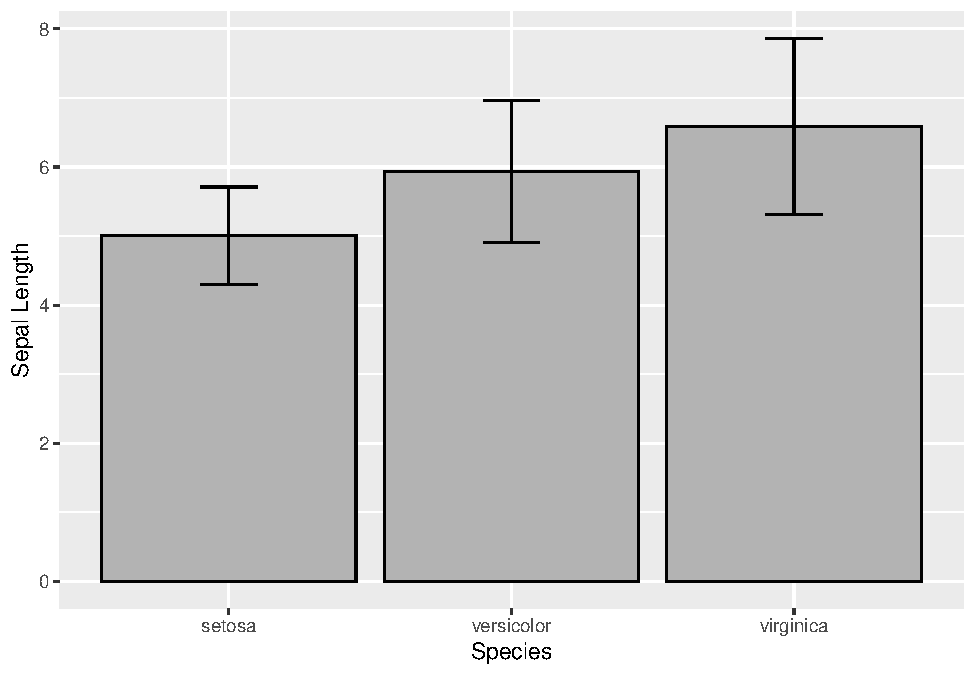
\includegraphics{module1_3_files/figure-latex/unnamed-chunk-15-1.pdf}

And for a slightly more complex example, let's consider the built in
\texttt{ToothGrowth} data set, which looks at tooth growth in guinea
pigs under three different vitamin C doses and two different delivery
methods (orange juice or ascorbic acid).

\begin{Shaded}
\begin{Highlighting}[]
\CommentTok{\# ?ToothGrowth}
\FunctionTok{head}\NormalTok{(ToothGrowth)}
\end{Highlighting}
\end{Shaded}

\begin{Shaded}
\begin{Highlighting}[]
\CommentTok{\# toothgrowth plot }


\NormalTok{ToothGrowth}\SpecialCharTok{$}\NormalTok{dose }\OtherTok{\textless{}{-}} \FunctionTok{as.factor}\NormalTok{(ToothGrowth}\SpecialCharTok{$}\NormalTok{dose)}

\NormalTok{sumTC }\OtherTok{\textless{}{-}}\NormalTok{ ToothGrowth }\SpecialCharTok{\%\textgreater{}\%} 
  \FunctionTok{group\_by}\NormalTok{(supp,dose) }\SpecialCharTok{\%\textgreater{}\%} 
  \FunctionTok{summarize}\NormalTok{(}\AttributeTok{mean =} \FunctionTok{mean}\NormalTok{(len),}
            \AttributeTok{sd =} \FunctionTok{sd}\NormalTok{(len))}


\NormalTok{p}\OtherTok{\textless{}{-}} \FunctionTok{ggplot}\NormalTok{(sumTC, }\FunctionTok{aes}\NormalTok{(}\AttributeTok{x=}\NormalTok{dose, }\AttributeTok{y=}\NormalTok{mean, }\AttributeTok{fill=}\NormalTok{supp)) }\SpecialCharTok{+} 
  \FunctionTok{geom\_col}\NormalTok{(}\AttributeTok{color=}\StringTok{"black"}\NormalTok{, }
           \AttributeTok{position=}\FunctionTok{position\_dodge}\NormalTok{()) }\SpecialCharTok{+}
  \FunctionTok{geom\_errorbar}\NormalTok{(}\FunctionTok{aes}\NormalTok{(}\AttributeTok{ymin=}\NormalTok{mean}\SpecialCharTok{{-}}\NormalTok{sd, }\AttributeTok{ymax=}\NormalTok{mean}\SpecialCharTok{+}\NormalTok{sd), }\AttributeTok{width=}\NormalTok{.}\DecValTok{2}\NormalTok{,}
                 \AttributeTok{position=}\FunctionTok{position\_dodge}\NormalTok{(}\FloatTok{0.9}\NormalTok{)) }\SpecialCharTok{+}
  \FunctionTok{labs}\NormalTok{(}\AttributeTok{title=}\StringTok{"Tooth growth"}\NormalTok{, }\AttributeTok{x=}\StringTok{"Dose (mg)"}\NormalTok{, }\AttributeTok{y =} \StringTok{"Length"}\NormalTok{) }\SpecialCharTok{+}
   \FunctionTok{theme\_classic}\NormalTok{() }\SpecialCharTok{+}
   \FunctionTok{scale\_fill\_manual}\NormalTok{(}\AttributeTok{values=}\FunctionTok{c}\NormalTok{(}\StringTok{\textquotesingle{}\#999999\textquotesingle{}}\NormalTok{,}\StringTok{\textquotesingle{}\#E69F00\textquotesingle{}}\NormalTok{))}

\FunctionTok{print}\NormalTok{(p)}
\end{Highlighting}
\end{Shaded}

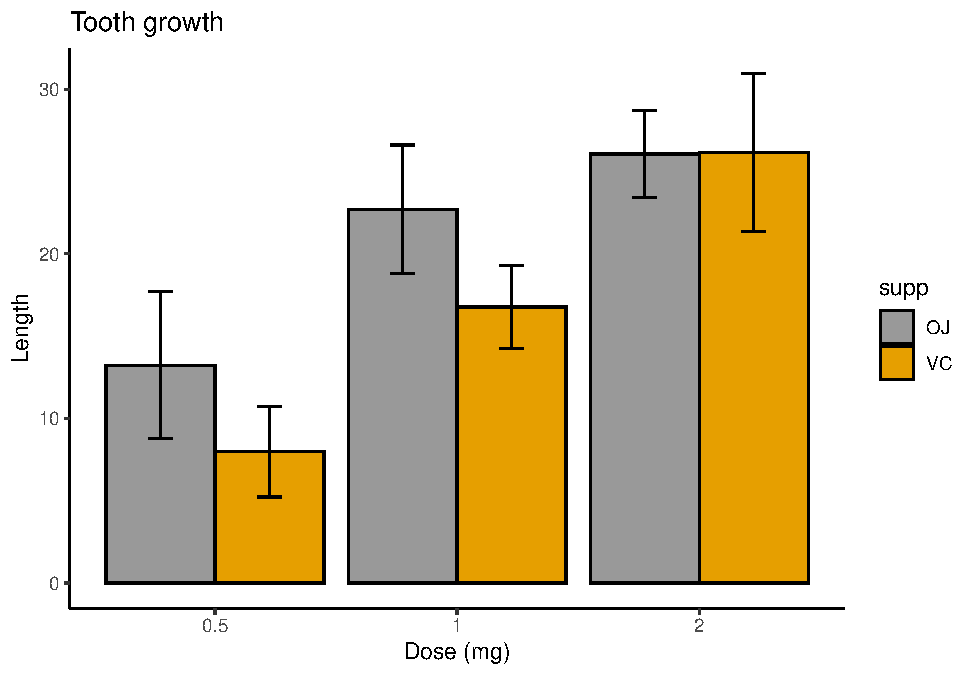
\includegraphics{module1_3_files/figure-latex/unnamed-chunk-16-1.pdf}

\hypertarget{beyond-ggplot}{%
\subsection{Beyond ggplot}\label{beyond-ggplot}}

ggplot contains an incredibly rich and powerful set of tools for
visualizing data. But ggplot and base R are not your only options! A
variety of packages exist for visualization, including:

\hypertarget{ggplot-extensions}{%
\subsubsection{ggplot extensions}\label{ggplot-extensions}}

Several packages have been created that build off of ggplot's syntax
with additional functions. You can find a list of them
\href{https://exts.ggplot2.tidyverse.org/gallery/}{here}.

\hypertarget{interactive-plots-leaflet-and-plotly}{%
\subparagraph{Interactive plots: leaflet and
plotly}\label{interactive-plots-leaflet-and-plotly}}

Increasingly, scientific journals are providing platforms for
interactive graphics on their websites to accompany published articles.
Interactive plots are also popular for personal, lab, and organizational
websites, and they can provide another option for your own data
exploration. Two of the most popular in R are
\href{https://plot.ly/r/}{plotly}, which offers a huge variety of 2D and
3D plots, and \href{https://rstudio.github.io/leaflet/}{leaflet}, which
is specifically for mapping.

Here's a quick and simple example of leaflet in action using the
``possumsites'' dataframe that accompanies the ``possum'' dataset in the
DAAG package. The dataset contains body measurements of several possums
in Australia. Where did they catch these possums?

\begin{Shaded}
\begin{Highlighting}[]
\CommentTok{\# use leaflet for interactive mapping! {-}{-}{-}{-}{-}{-}{-}{-}{-}{-}{-}{-}}

\FunctionTok{leaflet}\NormalTok{(possumsites) }\SpecialCharTok{\%\textgreater{}\%}
  \FunctionTok{addTiles}\NormalTok{() }\SpecialCharTok{\%\textgreater{}\%} \CommentTok{\#Adds map tiles from OpenStreetMap}
  \FunctionTok{addMarkers}\NormalTok{(}\AttributeTok{lng=}\FunctionTok{c}\NormalTok{(possumsites}\SpecialCharTok{$}\NormalTok{Longitude), }\AttributeTok{lat=}\FunctionTok{c}\NormalTok{(possumsites}\SpecialCharTok{$}\NormalTok{Latitude), }
             \AttributeTok{popup=}\FunctionTok{c}\NormalTok{(}\FunctionTok{as.character}\NormalTok{(possumsites}\SpecialCharTok{$}\NormalTok{altitude))) }\CommentTok{\#Adds markers for the sites}
\end{Highlighting}
\end{Shaded}

\hypertarget{challenge-exercises}{%
\subsection{Challenge exercises}\label{challenge-exercises}}

\begin{enumerate}
\def\labelenumi{\arabic{enumi}.}
\tightlist
\item
  Using the built in `mtcars' dataset, make a scatterplot of `mpg' as a
  function of `disp'. Color the points according to the `cyl' variable,
  and make the size of points vary depending on the `hp' variable. Try
  to code the `cyl' variable as a categorical variable (factor). The
  plot should look something like this:
\end{enumerate}

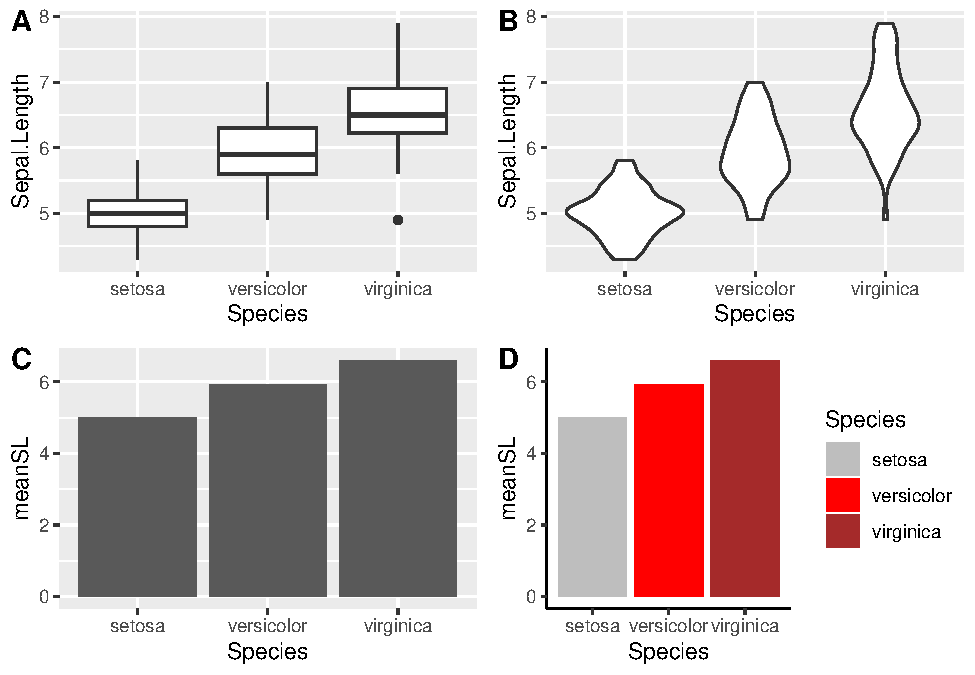
\includegraphics{module1_3_files/figure-latex/unnamed-chunk-18-1.pdf}

\begin{enumerate}
\def\labelenumi{\arabic{enumi}.}
\setcounter{enumi}{1}
\tightlist
\item
  Again using the `mtcars' data, make a scatterplot of `mpg' as a
  function of `disp'. Color the points according to the `cyl' variable,
  and make a separate trendline for each unique value of the `cyl'
  variable (with trendlines also indicating the `cyl' variable with the
  appropriate color).
\end{enumerate}

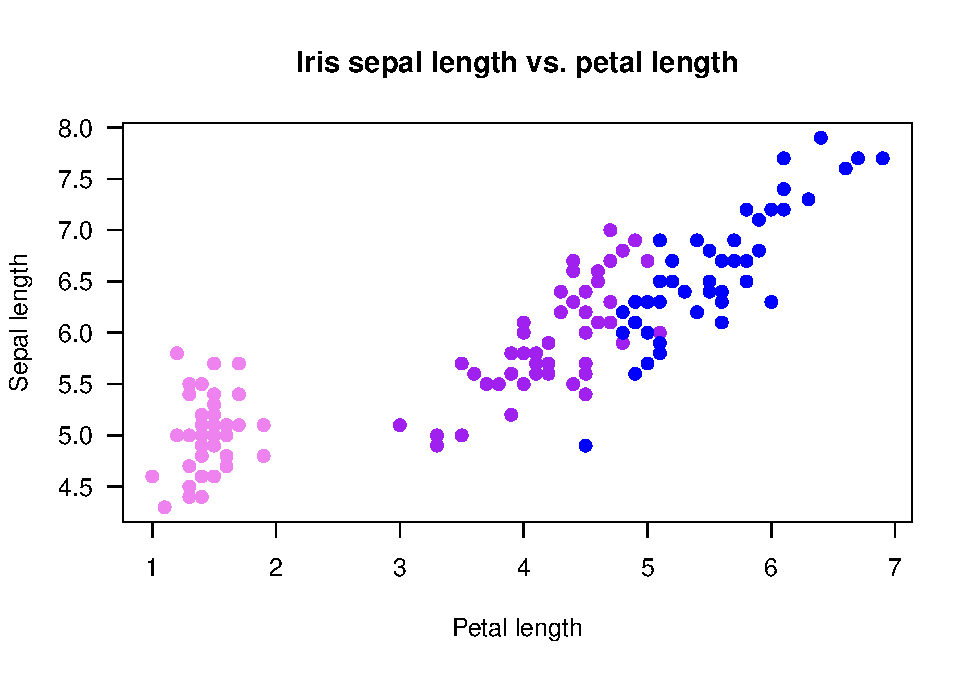
\includegraphics{module1_3_files/figure-latex/unnamed-chunk-19-1.pdf}

\begin{Shaded}
\begin{Highlighting}[]
\CommentTok{\# CHALLENGE EXERCISES   {-}{-}{-}{-}{-}{-}{-}{-}{-}{-}{-}{-}{-}{-}{-}{-}{-}{-}{-}{-}{-}{-}{-}{-}{-}{-}{-}{-}{-}{-}{-}{-}{-}{-}{-}{-}{-}}

\CommentTok{\# 1. Using the built in \textquotesingle{}mtcars\textquotesingle{} dataset, make a scatterplot of \textquotesingle{}mpg\textquotesingle{} as a function of \textquotesingle{}disp\textquotesingle{}. Color the points}
\CommentTok{\# according to the \textquotesingle{}cyl\textquotesingle{} variable, and make the size of points vary depending on the \textquotesingle{}hp\textquotesingle{} variable. Try to code}
\CommentTok{\# the \textquotesingle{}cyl\textquotesingle{} variable as a categorical variable (factor). The plot should look something like this:}
\CommentTok{\#}
\CommentTok{\# 2. Again using the \textquotesingle{}mtcars\textquotesingle{} data, make a scatterplot of \textquotesingle{}mpg\textquotesingle{} as a function of \textquotesingle{}disp\textquotesingle{}. Color the points}
\CommentTok{\# according to the \textquotesingle{}cyl\textquotesingle{} variable, and make a separate trendline for each unique value of the \textquotesingle{}cyl\textquotesingle{} variable (with}
\CommentTok{\# trendlines also indicating the \textquotesingle{}cyl\textquotesingle{} variable with the appropriate color). }
\end{Highlighting}
\end{Shaded}

\href{module1_4.html}{--go to next submodule--}

\hypertarget{more-advanced-ggplot-demo-optional}{%
\subsection{More advanced GGplot demo
(optional!)}\label{more-advanced-ggplot-demo-optional}}

For additional practice, let's use the Soils dataset from the `carData'
package, which contains soil attributes from a gilgai landscape (mounds
and depressions caused by shrinking and swelling of clays during dry and
wet seasons) in Australia.

First we will need to load a few more packages. Make sure to install any
packages in this list you don't already have!

\begin{Shaded}
\begin{Highlighting}[]
\CommentTok{\# More complex demo {-}{-}{-}{-}{-}{-}{-}{-}{-}{-}{-}{-}{-}{-}{-}{-}{-}{-}{-}{-}{-}{-}{-}{-}{-}{-}{-}{-}{-}}

\FunctionTok{library}\NormalTok{(ggthemes)}
\FunctionTok{library}\NormalTok{(carData)}
\FunctionTok{library}\NormalTok{(DAAG)}
\FunctionTok{library}\NormalTok{(RColorBrewer)}
\end{Highlighting}
\end{Shaded}

Now load the dataset.

\begin{Shaded}
\begin{Highlighting}[]
\CommentTok{\# Load the example data }

\NormalTok{soil }\OtherTok{\textless{}{-}}\NormalTok{ carData}\SpecialCharTok{::}\NormalTok{Soils    }\CommentTok{\# load example data}

\CommentTok{\#See what variables it contains...}
\FunctionTok{head}\NormalTok{(soil)    }\CommentTok{\# plot out the first few lines...}
\end{Highlighting}
\end{Shaded}

Staring simply, let's say we're interested in how pH, a continuous
variable, varies with contour position, a categorical factor:

\begin{Shaded}
\begin{Highlighting}[]
\CommentTok{\# basic boxplot and violin plot}

\NormalTok{plot1 }\OtherTok{\textless{}{-}} \FunctionTok{ggplot}\NormalTok{(soil) }\SpecialCharTok{+}
  \FunctionTok{geom\_boxplot}\NormalTok{(}\FunctionTok{aes}\NormalTok{(}\AttributeTok{x=}\NormalTok{Contour, }\AttributeTok{y=}\NormalTok{pH))}

\NormalTok{plot2 }\OtherTok{\textless{}{-}} \FunctionTok{ggplot}\NormalTok{(soil) }\SpecialCharTok{+} 
  \FunctionTok{geom\_violin}\NormalTok{(}\FunctionTok{aes}\NormalTok{(}\AttributeTok{x=}\NormalTok{Contour, }\AttributeTok{y=}\NormalTok{pH))}

\FunctionTok{plot\_grid}\NormalTok{(plot1,plot2,}\AttributeTok{labels =} \StringTok{"AUTO"}\NormalTok{)}
\end{Highlighting}
\end{Shaded}

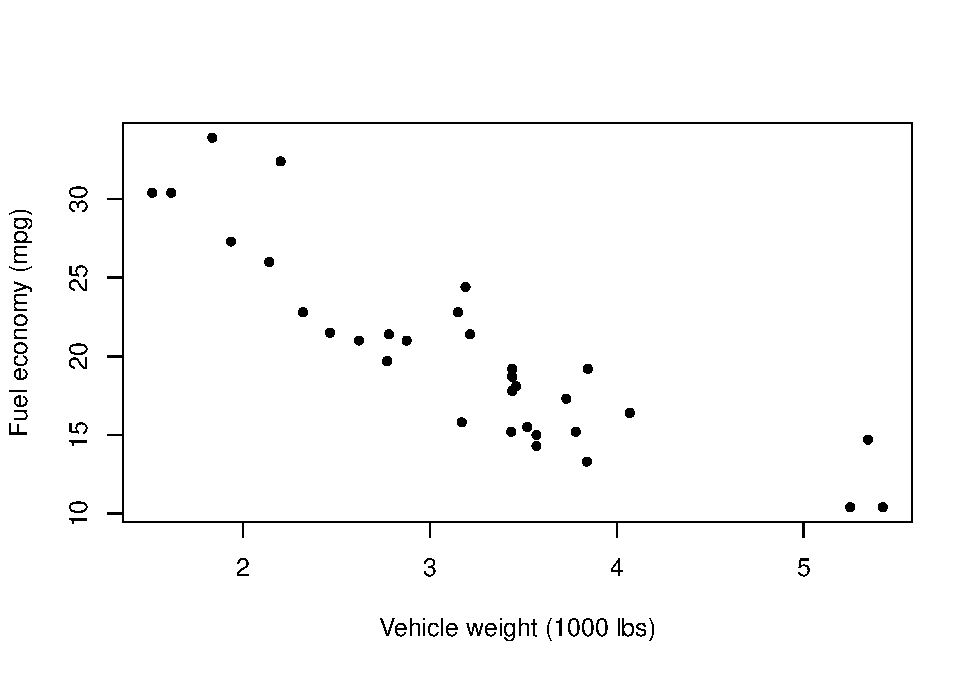
\includegraphics{module1_3_files/figure-latex/unnamed-chunk-24-1.pdf}

Next let's try a simple scatterplot of two continuous variables, Calcium
content and pH:

\begin{Shaded}
\begin{Highlighting}[]
\CommentTok{\# basic scatterplot}

\FunctionTok{ggplot}\NormalTok{(soil) }\SpecialCharTok{+}
  \FunctionTok{geom\_point}\NormalTok{(}\FunctionTok{aes}\NormalTok{(}\AttributeTok{x=}\NormalTok{pH, }\AttributeTok{y=}\NormalTok{Ca))}
\end{Highlighting}
\end{Shaded}

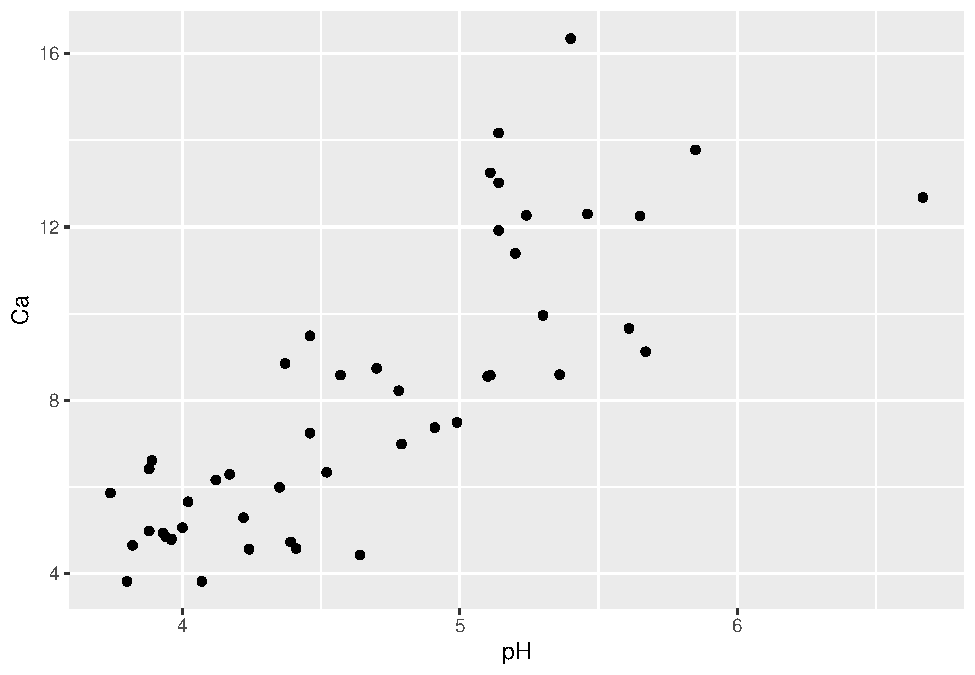
\includegraphics{module1_3_files/figure-latex/unnamed-chunk-25-1.pdf}

Now let's say you wanted to examine if/how the relationship between pH
and Ca varies with depth. You could go back to your scatterplot and use
color to identify points from the different sampling depths.

\begin{Shaded}
\begin{Highlighting}[]
\CommentTok{\# Color the points by depth}

\FunctionTok{ggplot}\NormalTok{(soil) }\SpecialCharTok{+}
  \FunctionTok{geom\_point}\NormalTok{(}\FunctionTok{aes}\NormalTok{(}\AttributeTok{x=}\NormalTok{pH, }\AttributeTok{y=}\NormalTok{Ca, }\AttributeTok{color=}\NormalTok{Depth))}
\end{Highlighting}
\end{Shaded}

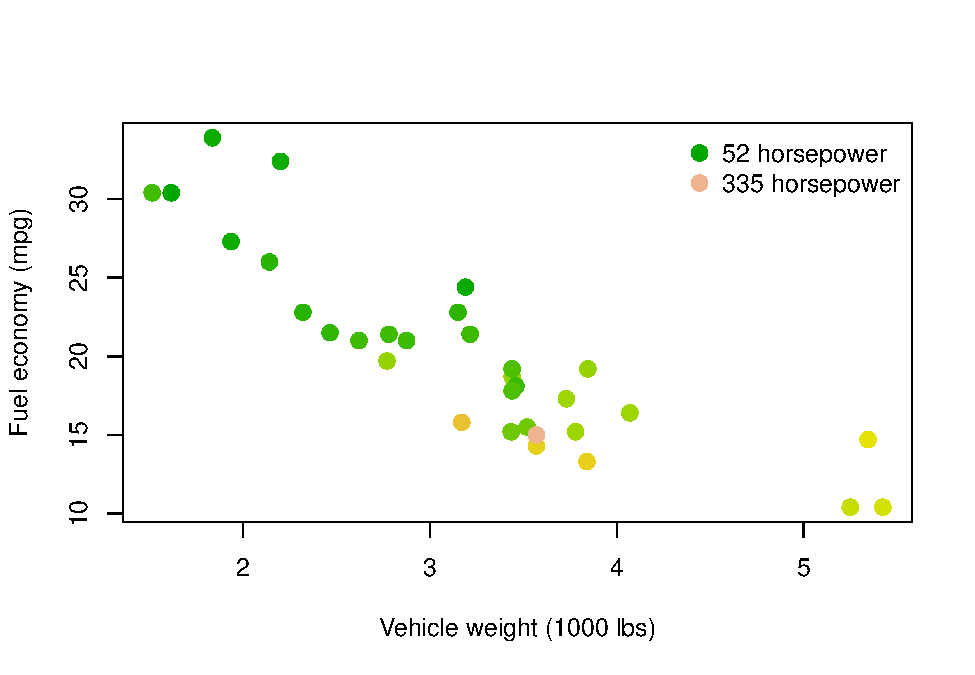
\includegraphics{module1_3_files/figure-latex/unnamed-chunk-26-1.pdf}

Try playing around with applying a few graphical attributes to all the
points (specified outside the \texttt{aes()} argument). Try specifying
\texttt{shape=21}, \texttt{color="black"} , \texttt{size=3} and
\texttt{stroke=1}:

\begin{Shaded}
\begin{Highlighting}[]
\CommentTok{\# make additional alterations (outside the "aes" function)}

\FunctionTok{ggplot}\NormalTok{(soil) }\SpecialCharTok{+}
  \FunctionTok{geom\_point}\NormalTok{(}\FunctionTok{aes}\NormalTok{(}\AttributeTok{x=}\NormalTok{pH, }\AttributeTok{y=}\NormalTok{Ca, }\AttributeTok{fill=}\NormalTok{Depth), }\AttributeTok{shape=}\DecValTok{21}\NormalTok{, }\AttributeTok{color=}\StringTok{"black"}\NormalTok{, }\AttributeTok{size=}\DecValTok{4}\NormalTok{, }\AttributeTok{stroke=}\FloatTok{1.5}\NormalTok{)}
\end{Highlighting}
\end{Shaded}

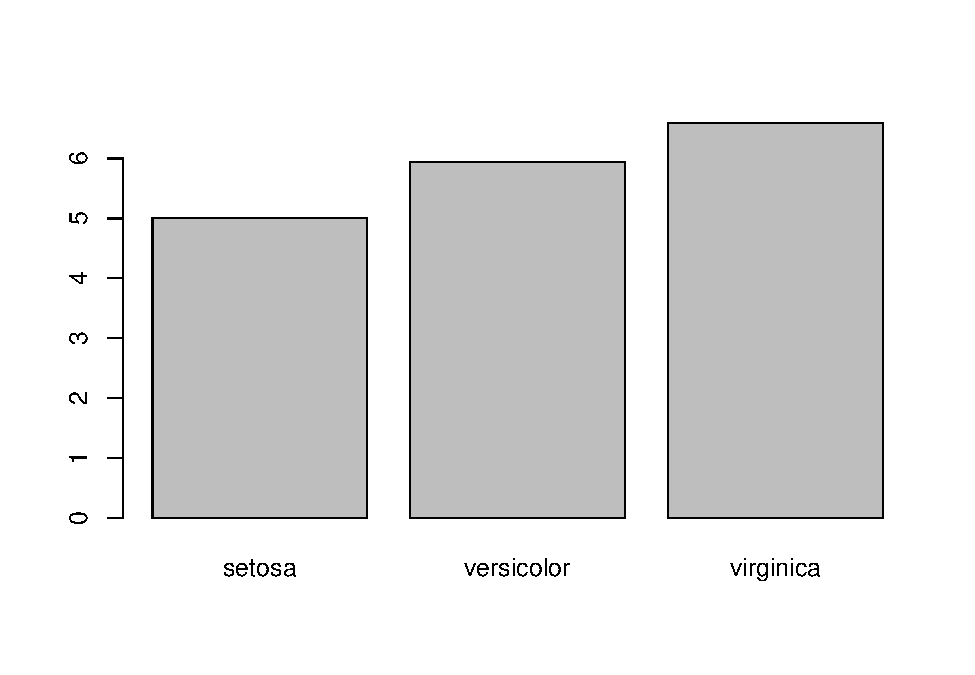
\includegraphics{module1_3_files/figure-latex/unnamed-chunk-27-1.pdf}

Now for something new: let's plot relationships between pH and several
soil nutrients on the same graph. Notice that the y axis label defaults
to the first set of points (Ca), and we'd need to modify it. Also there
is no legend! You'd have to change things like axis labels and legend
titles `manually' to complete this figure.

\begin{Shaded}
\begin{Highlighting}[]
\CommentTok{\# Plot several relationships on same plot}

\FunctionTok{ggplot}\NormalTok{(soil, }\FunctionTok{aes}\NormalTok{(}\AttributeTok{x=}\NormalTok{pH)) }\SpecialCharTok{+}
  \FunctionTok{geom\_point}\NormalTok{(}\FunctionTok{aes}\NormalTok{(}\AttributeTok{y=}\NormalTok{Ca), }\AttributeTok{shape=}\DecValTok{21}\NormalTok{, }\AttributeTok{fill=}\StringTok{"red"}\NormalTok{, }\AttributeTok{color=}\StringTok{"black"}\NormalTok{, }\AttributeTok{size=}\DecValTok{4}\NormalTok{, }\AttributeTok{stroke=}\FloatTok{1.5}\NormalTok{) }\SpecialCharTok{+}
  \FunctionTok{geom\_point}\NormalTok{(}\FunctionTok{aes}\NormalTok{(}\AttributeTok{y=}\NormalTok{Mg), }\AttributeTok{shape=}\DecValTok{21}\NormalTok{, }\AttributeTok{fill=}\StringTok{"blue"}\NormalTok{, }\AttributeTok{color=}\StringTok{"black"}\NormalTok{, }\AttributeTok{size=}\DecValTok{4}\NormalTok{, }\AttributeTok{stroke=}\FloatTok{1.5}\NormalTok{) }\SpecialCharTok{+}
  \FunctionTok{geom\_point}\NormalTok{(}\FunctionTok{aes}\NormalTok{(}\AttributeTok{y=}\NormalTok{Na), }\AttributeTok{shape=}\DecValTok{21}\NormalTok{, }\AttributeTok{fill=}\StringTok{"gray30"}\NormalTok{, }\AttributeTok{color=}\StringTok{"black"}\NormalTok{, }\AttributeTok{size=}\DecValTok{4}\NormalTok{, }\AttributeTok{stroke=}\FloatTok{1.5}\NormalTok{)}
\end{Highlighting}
\end{Shaded}

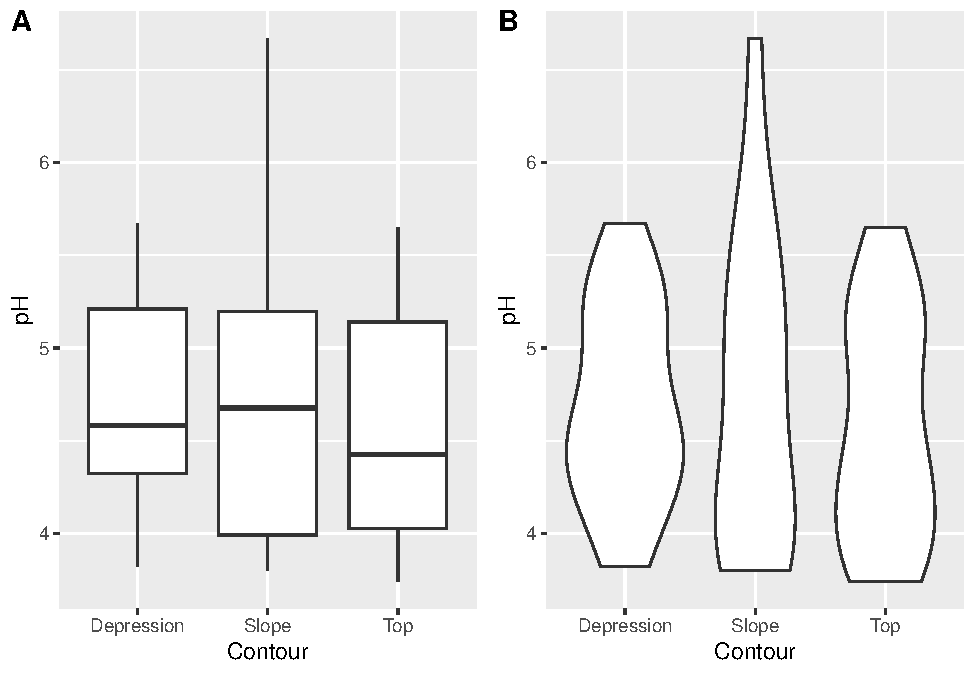
\includegraphics{module1_3_files/figure-latex/unnamed-chunk-28-1.pdf}

There's a better way to do it. But first we need to `reshape' our soils
data with the tidyverse function `pivot\_longer().

\hypertarget{aside-tidy-data-and-reshaping-functions}{%
\subsubsection{ASIDE: tidy data and reshaping
functions}\label{aside-tidy-data-and-reshaping-functions}}

All of the tidyverse set of packages are designed to work with
\emph{Tidy} formatted data.

This means:

\begin{itemize}
\tightlist
\item
  Each variable must have its own column.
\item
  Each observation must have its own row.
\item
  Each value must have its own cell.
\end{itemize}

This is what it looks like:

\includegraphics{tidy-1.png}

The \emph{tidyr} package has several functions to help you get your data
into this format.

Use ``pivot\_longer()'' to get all of the values and variables from
multiple columns into a single column.

\includegraphics{tidy-9.png}

Use ``pivot\_wider()'' to distribute two variables in a single column
into separate columns, with their data values(`value')

\includegraphics{tidy-8.png}

For a nice intro to `pivot\_wider' and `pivot\_longer', see
\href{https://tidyr.tidyverse.org/articles/pivot.html}{this link}

\hypertarget{back-to-the-example}{%
\subsubsection{Back to the example\ldots{}}\label{back-to-the-example}}

Let's reshape the soil dataset into the long format- which in this case
treats each separate nutrient measurement as a different observation
(row).

\begin{Shaded}
\begin{Highlighting}[]
\CommentTok{\# Use \textquotesingle{}tidyverse\textquotesingle{} to reshape the data }

\NormalTok{soil.nut }\OtherTok{\textless{}{-}} \FunctionTok{pivot\_longer}\NormalTok{(soil, }\AttributeTok{cols=}\FunctionTok{c}\NormalTok{(}\StringTok{"Ca"}\NormalTok{,}\StringTok{"Mg"}\NormalTok{,}\StringTok{"Na"}\NormalTok{), }\AttributeTok{names\_to=}\StringTok{"nutrient"}\NormalTok{,}\AttributeTok{values\_to =} \StringTok{"value"}\NormalTok{ )}
\NormalTok{soil.nut}
\end{Highlighting}
\end{Shaded}

This lets us plot our different nutrients as factor levels without
typing each one with its specifications on its own line, and
automatically generates a legend that identifies the series (and also
gives the default ggplot colors).

\begin{Shaded}
\begin{Highlighting}[]
\FunctionTok{ggplot}\NormalTok{(soil.nut) }\SpecialCharTok{+}
  \FunctionTok{geom\_point}\NormalTok{(}\FunctionTok{aes}\NormalTok{(}\AttributeTok{x=}\NormalTok{pH, }\AttributeTok{y=}\NormalTok{value, }\AttributeTok{fill=}\NormalTok{nutrient), }\AttributeTok{shape=}\DecValTok{21}\NormalTok{, }\AttributeTok{color=}\StringTok{"black"}\NormalTok{, }\AttributeTok{size=}\DecValTok{4}\NormalTok{, }\AttributeTok{stroke=}\FloatTok{1.5}\NormalTok{)}
\end{Highlighting}
\end{Shaded}

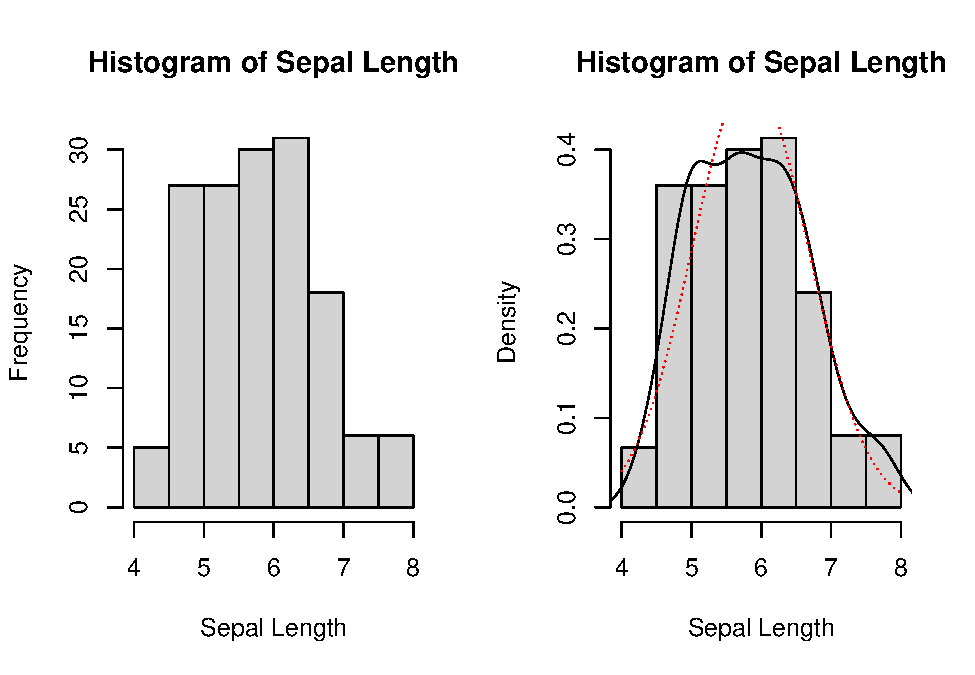
\includegraphics{module1_3_files/figure-latex/unnamed-chunk-30-1.pdf}

What if instead of Na, we had K as our third nutrient of interest?

\begin{Shaded}
\begin{Highlighting}[]
\CommentTok{\# or if we wanted to plot different nutrients...}

\NormalTok{soil.nut2 }\OtherTok{\textless{}{-}} \FunctionTok{pivot\_longer}\NormalTok{(soil, }\AttributeTok{cols=}\FunctionTok{c}\NormalTok{(}\StringTok{"Ca"}\NormalTok{,}\StringTok{"Mg"}\NormalTok{,}\StringTok{"K"}\NormalTok{), }\AttributeTok{names\_to=}\StringTok{"nutrient"}\NormalTok{,}\AttributeTok{values\_to =} \StringTok{"value"}\NormalTok{ )}

\FunctionTok{ggplot}\NormalTok{(soil.nut2) }\SpecialCharTok{+}
  \FunctionTok{geom\_point}\NormalTok{(}\FunctionTok{aes}\NormalTok{(}\AttributeTok{x=}\NormalTok{pH, }\AttributeTok{y=}\NormalTok{value, }\AttributeTok{fill=}\NormalTok{nutrient), }\AttributeTok{shape=}\DecValTok{21}\NormalTok{, }\AttributeTok{color=}\StringTok{"black"}\NormalTok{, }\AttributeTok{size=}\DecValTok{4}\NormalTok{, }\AttributeTok{stroke=}\FloatTok{1.5}\NormalTok{)}
\end{Highlighting}
\end{Shaded}

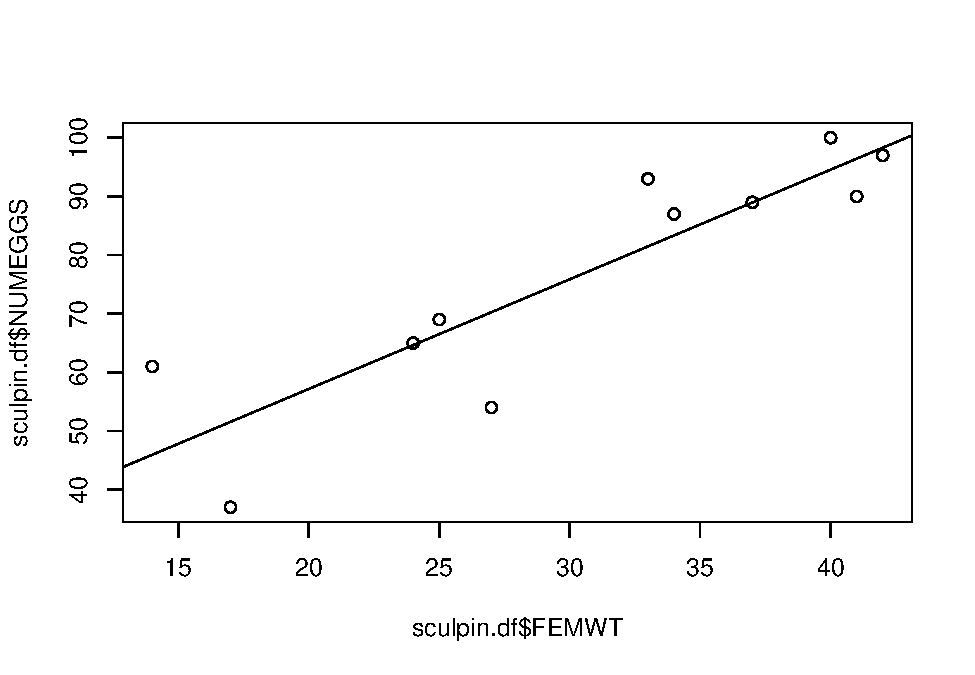
\includegraphics{module1_3_files/figure-latex/unnamed-chunk-31-1.pdf}

The problem here is that K occurs at natural concentrations that differ
from the other nutrients by an order of magnitude, so it's difficult to
examine them all on the same scale. One approach we can take is to plot
them separately. While we're at it, let's also make sure that we specify
the response units on the y-axis.

\hypertarget{facets-and-scales-and-themes}{%
\subsubsection{Facets and scales, and
themes}\label{facets-and-scales-and-themes}}

The next plot introduces:

\begin{itemize}
\item
  \textbf{facets}, which allow you to display data on separate panels
  using some grouping variable
\item
  \textbf{scales}, which allow you to adjust how to represent the data
  with axes and colors
\end{itemize}

We also play around with some more ggplot \emph{themes}.

\begin{Shaded}
\begin{Highlighting}[]
\CommentTok{\# plot with facets, scales, and themes!}

\FunctionTok{ggplot}\NormalTok{(soil.nut2) }\SpecialCharTok{+}
  \FunctionTok{geom\_point}\NormalTok{(}\FunctionTok{aes}\NormalTok{(}\AttributeTok{x=}\NormalTok{pH, }\AttributeTok{y=}\NormalTok{value, }\AttributeTok{fill=}\NormalTok{nutrient), }
             \AttributeTok{shape=}\DecValTok{21}\NormalTok{, }\AttributeTok{color=}\StringTok{"black"}\NormalTok{, }\AttributeTok{size=}\DecValTok{4}\NormalTok{, }\AttributeTok{stroke=}\FloatTok{1.5}\NormalTok{) }\SpecialCharTok{+}
  \FunctionTok{facet\_wrap}\NormalTok{(}\SpecialCharTok{\textasciitilde{}}\NormalTok{nutrient, }\AttributeTok{scales=}\StringTok{"free\_y"}\NormalTok{) }\SpecialCharTok{+}
  \FunctionTok{labs}\NormalTok{(}\AttributeTok{y=}\StringTok{"mg / 100 g soil"}\NormalTok{) }\SpecialCharTok{+}
  \FunctionTok{theme\_bw}\NormalTok{() }\SpecialCharTok{+}
  \FunctionTok{theme}\NormalTok{(}\AttributeTok{legend.position=}\StringTok{"none"}\NormalTok{,}
        \AttributeTok{axis.text =} \FunctionTok{element\_text}\NormalTok{(}\AttributeTok{size=}\DecValTok{20}\NormalTok{),}
        \AttributeTok{axis.title =} \FunctionTok{element\_text}\NormalTok{(}\AttributeTok{size=}\DecValTok{25}\NormalTok{),}
        \AttributeTok{strip.text =} \FunctionTok{element\_text}\NormalTok{(}\AttributeTok{size=}\DecValTok{25}\NormalTok{, }\AttributeTok{face=}\StringTok{"bold"}\NormalTok{))}
\end{Highlighting}
\end{Shaded}

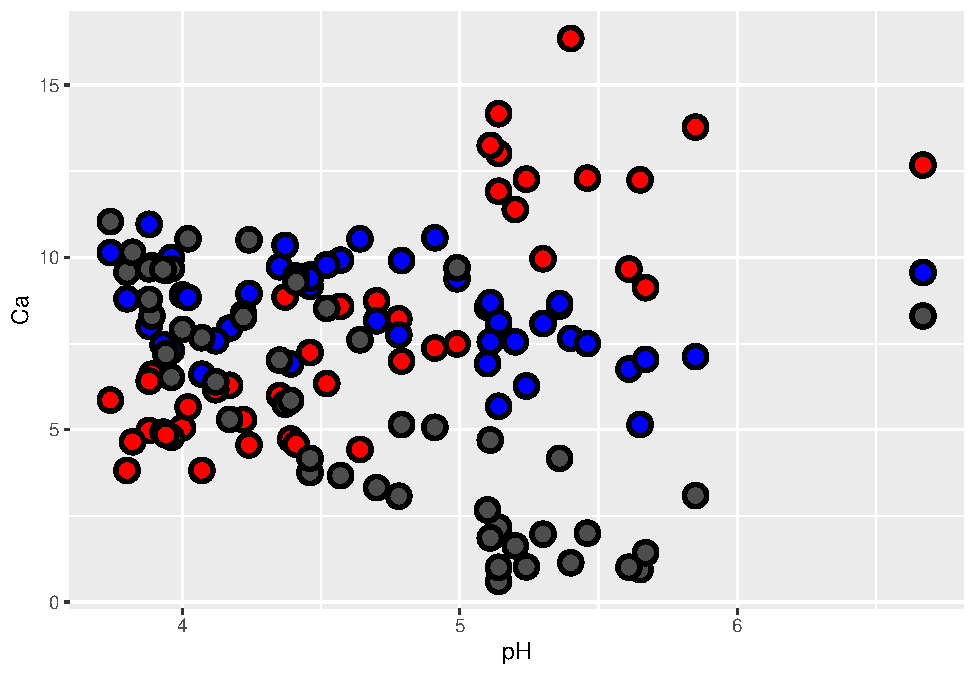
\includegraphics{module1_3_files/figure-latex/unnamed-chunk-32-1.pdf}

In this plot, we've kept the different colors for each nutrient, but
suppressed the legend that is auto-generated by ggplot, because this
information is now redundant with the headers of the three facets. In
the \textbf{\texttt{facet\_wrap}} function, we used
\textbf{\texttt{scales}} to specify that the y-axis should be bounded to
fit the data within each facet. There are some cases where you would
probably want the axes to be the same -- e.g.~if you were comparing raw
values across groups, rather than the distributions or trends of the
data.

We also changed the theme. ggplot has
\href{http://r4ds.had.co.nz/images/visualization-themes.png}{8 built-in
themes} to choose from. There are also lots of other themes built into
extension packages such as ggthemes.

You can also fine-tune pretty much any of the details (gridlines or no?
plot borders? line weight of the borders and gridlines? axis label
angles?) to your heart's content using the arguments in the
\textbf{\texttt{theme()}} function.

\hypertarget{aside-specifying-colors}{%
\subsubsection{ASIDE: Specifying colors}\label{aside-specifying-colors}}

Sometimes sticking to the default colors in ggplot isn't the best
choice. You might have factors representing ordered ranks, like in an
experiment with different levels of light exposure, and want to
represent these levels on a monochromatic scale. Or you might want to
make a map displaying regions of positive or negative change in forest
cover, using a diverging color scale. Or you don't even like the default
ggplot colors, and have your own preferred color schemes. It's also
important to remember that red-green colorblindness is fairly common, so
if you are presenting data that must be distinguished by colors in a
single plotting area, you should probably avoid this combination or
combine it with changes in value (light to dark) in order for your plot
to be accessible.

Going back to our earlier example showing Ca content by pH at different
depths, let's say we want a color scheme where deeper depths are
represented by darker values of the same color. We can do this by using
another scale function.

One method is to use \textbf{\texttt{scale\_fill\_brewer}}, and select
an already composed color palette from RColorBrewer (a package you'll
need to install). You can check out all of the options available in
RColorBrewer by entering \textbf{\texttt{display.brewer.all()}}, which
shows the sequential palettes, then categorical palettes, than diverging
palettes.

\begin{Shaded}
\begin{Highlighting}[]
\CommentTok{\# Playing with colors in ggplot!}

\FunctionTok{display.brewer.all}\NormalTok{()}
\end{Highlighting}
\end{Shaded}

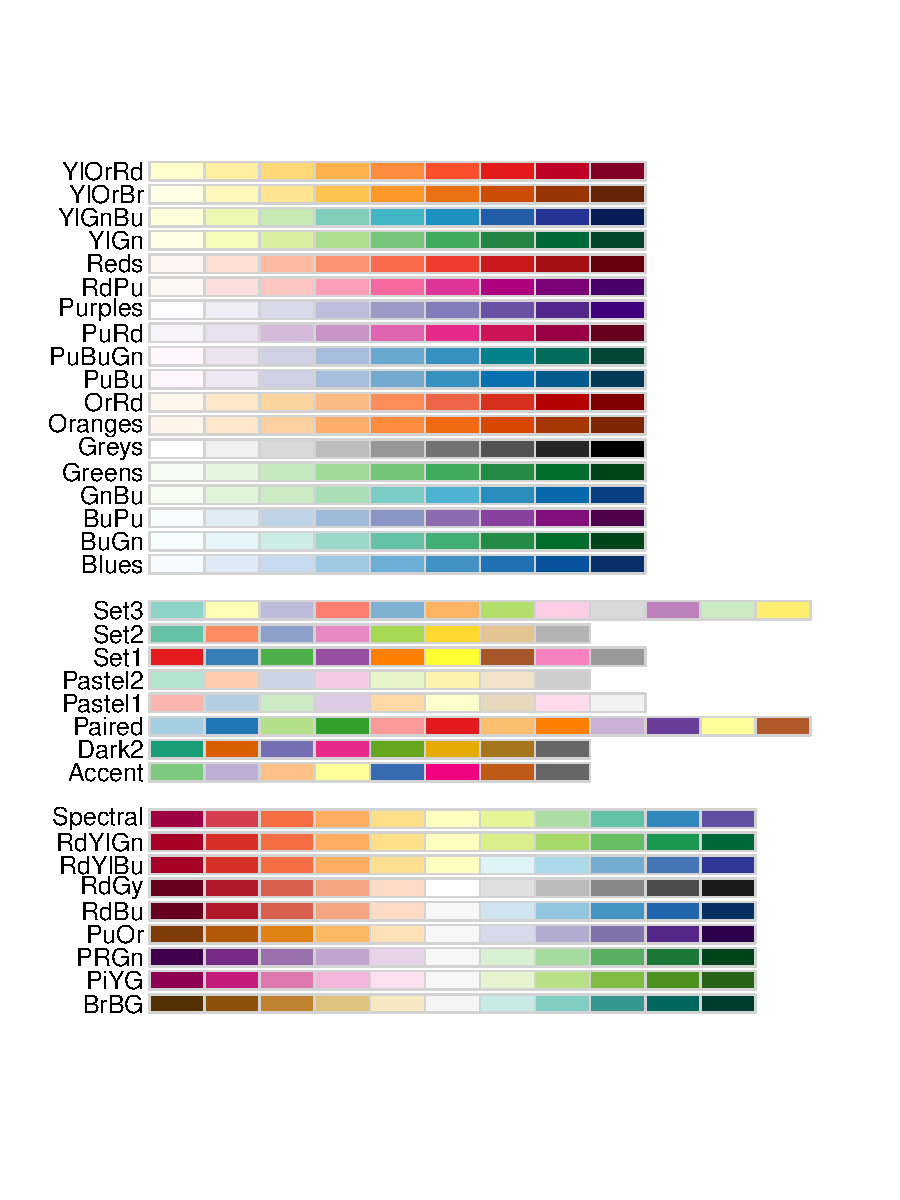
\includegraphics{module1_3_files/figure-latex/unnamed-chunk-33-1.pdf}

I'm going to pick the YlOrBr (Yellow-Orange-Brown) palette, because
those seem like good soil-y colors. Notice that because
\textbf{\texttt{fill}} is mapped to the values of the data, inside this
function is where I can change the title of the legend (and the labels
for the different values, if I wanted to do that).

\begin{Shaded}
\begin{Highlighting}[]
\CommentTok{\# Choose a new color palette from the RColorBrewer package}

\FunctionTok{ggplot}\NormalTok{(soil) }\SpecialCharTok{+}
  \FunctionTok{geom\_point}\NormalTok{(}\FunctionTok{aes}\NormalTok{(}\AttributeTok{x=}\NormalTok{pH, }\AttributeTok{y=}\NormalTok{Ca, }\AttributeTok{fill=}\NormalTok{Depth), }\AttributeTok{shape=}\DecValTok{21}\NormalTok{, }\AttributeTok{color=}\StringTok{"black"}\NormalTok{, }\AttributeTok{size=}\DecValTok{4}\NormalTok{, }\AttributeTok{stroke=}\FloatTok{1.5}\NormalTok{) }\SpecialCharTok{+}
  \FunctionTok{theme\_classic}\NormalTok{() }\SpecialCharTok{+}
  \FunctionTok{labs}\NormalTok{(}\AttributeTok{y=}\StringTok{"Ca (mg/100g soil)"}\NormalTok{) }\SpecialCharTok{+}
  \FunctionTok{scale\_fill\_brewer}\NormalTok{(}\AttributeTok{palette=}\StringTok{"YlOrBr"}\NormalTok{, }\AttributeTok{name=}\StringTok{"Depth (cm)"}\NormalTok{)}
\end{Highlighting}
\end{Shaded}

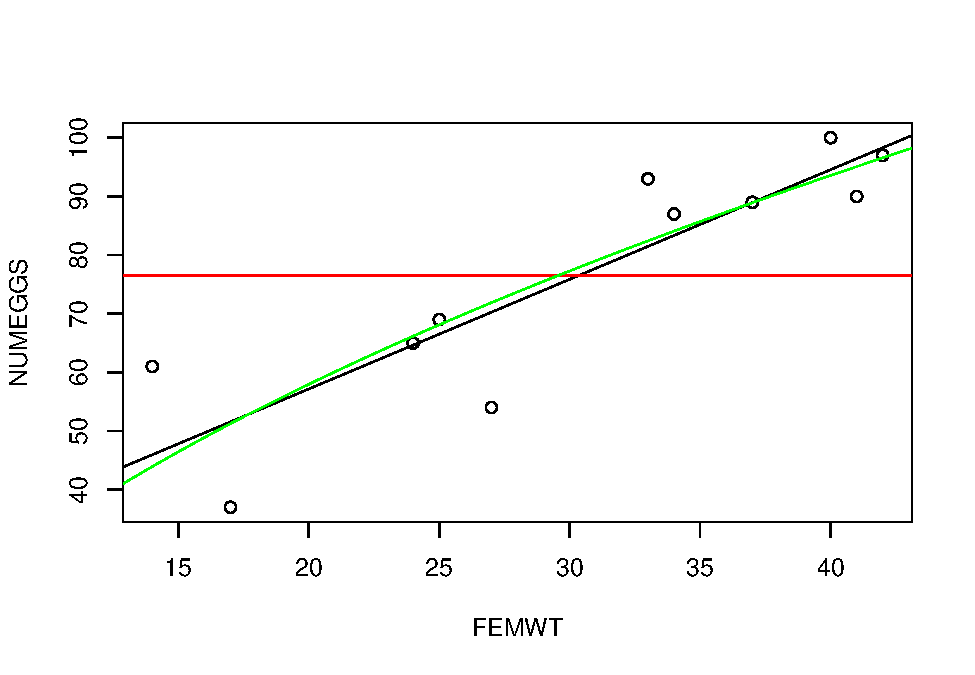
\includegraphics{module1_3_files/figure-latex/unnamed-chunk-34-1.pdf}

Another method is to use \textbf{\texttt{scale\_fill\_manual}}, with
which you define your own palette. To pick out your colors, you can use
the
\href{\textquotesingle{}http://www.stat.columbia.edu/~tzheng/files/Rcolor.pdf}{names
of colors} already recognized by R, or use
\href{https://htmlcolorcodes.com/}{hex codes} for any color you want.

\begin{Shaded}
\begin{Highlighting}[]
\CommentTok{\# Choose your own palette!}

\FunctionTok{ggplot}\NormalTok{(soil) }\SpecialCharTok{+}
  \FunctionTok{geom\_point}\NormalTok{(}\FunctionTok{aes}\NormalTok{(}\AttributeTok{x=}\NormalTok{pH, }\AttributeTok{y=}\NormalTok{Ca, }\AttributeTok{fill=}\NormalTok{Depth), }\AttributeTok{shape=}\DecValTok{21}\NormalTok{, }\AttributeTok{color=}\StringTok{"black"}\NormalTok{, }\AttributeTok{size=}\DecValTok{4}\NormalTok{, }\AttributeTok{stroke=}\FloatTok{1.5}\NormalTok{) }\SpecialCharTok{+}
  \FunctionTok{theme\_bw}\NormalTok{() }\SpecialCharTok{+}
  \FunctionTok{ylab}\NormalTok{(}\StringTok{"Ca (mg/100g soil)"}\NormalTok{) }\SpecialCharTok{+}
  \FunctionTok{scale\_fill\_manual}\NormalTok{(}\AttributeTok{values=}\FunctionTok{c}\NormalTok{(}\StringTok{"\#FFF0BF"}\NormalTok{,}\StringTok{"\#FFC300"}\NormalTok{,}\StringTok{"\#BF9200"}\NormalTok{,}\StringTok{"\#604900"}\NormalTok{), }\AttributeTok{name=}\StringTok{"Depth (cm)"}\NormalTok{)}
\end{Highlighting}
\end{Shaded}

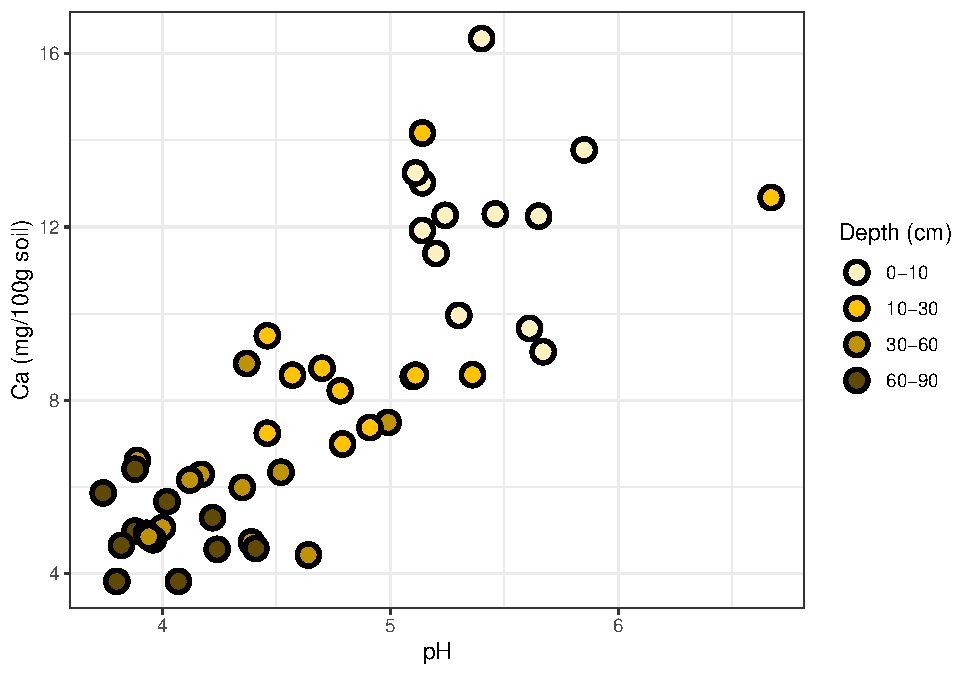
\includegraphics{module1_3_files/figure-latex/unnamed-chunk-35-1.pdf}

What if depth were a continuous variable, rather than a set of four
discrete categories? We could use
\textbf{\texttt{scale\_fill\_gradient}}, supply the hues we want (one
for monochromatic, two for diverging) and R would map the soil depth
values to color values along the gradient.

\hypertarget{trendlines}{%
\paragraph{Trendlines}\label{trendlines}}

Next, we might want to add a trendline to each set of points. Try it for
the plot we made of different nutrient concentrations as a function of
pH. Arguments in the \textbf{\texttt{geom\_smooth()}} function allow us
to change the confidence level, the smoothing method, and other details:

\begin{Shaded}
\begin{Highlighting}[]
\CommentTok{\# add trendlines}

\FunctionTok{ggplot}\NormalTok{(soil.nut2) }\SpecialCharTok{+}
  \FunctionTok{geom\_point}\NormalTok{(}\FunctionTok{aes}\NormalTok{(}\AttributeTok{x=}\NormalTok{pH, }\AttributeTok{y=}\NormalTok{value, }\AttributeTok{fill=}\NormalTok{nutrient), }
             \AttributeTok{shape=}\DecValTok{21}\NormalTok{, }\AttributeTok{color=}\StringTok{"black"}\NormalTok{, }\AttributeTok{size=}\DecValTok{4}\NormalTok{, }\AttributeTok{stroke=}\FloatTok{1.5}\NormalTok{) }\SpecialCharTok{+}
  \FunctionTok{geom\_smooth}\NormalTok{(}\FunctionTok{aes}\NormalTok{(}\AttributeTok{x=}\NormalTok{pH, }\AttributeTok{y=}\NormalTok{value), }\AttributeTok{method=}\StringTok{"lm"}\NormalTok{, }\AttributeTok{color=}\StringTok{"black"}\NormalTok{) }\SpecialCharTok{+}
  \FunctionTok{facet\_wrap}\NormalTok{(}\SpecialCharTok{\textasciitilde{}}\NormalTok{nutrient, }\AttributeTok{scales=}\StringTok{"free\_y"}\NormalTok{) }\SpecialCharTok{+}
  \FunctionTok{ylab}\NormalTok{(}\StringTok{"mg / 100 g soil"}\NormalTok{) }\SpecialCharTok{+}
  \FunctionTok{theme\_classic}\NormalTok{() }\SpecialCharTok{+}
  \FunctionTok{theme}\NormalTok{(}\AttributeTok{legend.position=}\StringTok{"none"}\NormalTok{,}
        \AttributeTok{axis.text =} \FunctionTok{element\_text}\NormalTok{(}\AttributeTok{size=}\DecValTok{14}\NormalTok{),}
        \AttributeTok{axis.title =} \FunctionTok{element\_text}\NormalTok{(}\AttributeTok{size=}\DecValTok{16}\NormalTok{),}
        \AttributeTok{strip.text =} \FunctionTok{element\_text}\NormalTok{(}\AttributeTok{size=}\DecValTok{16}\NormalTok{, }\AttributeTok{face=}\StringTok{"bold"}\NormalTok{))}
\end{Highlighting}
\end{Shaded}

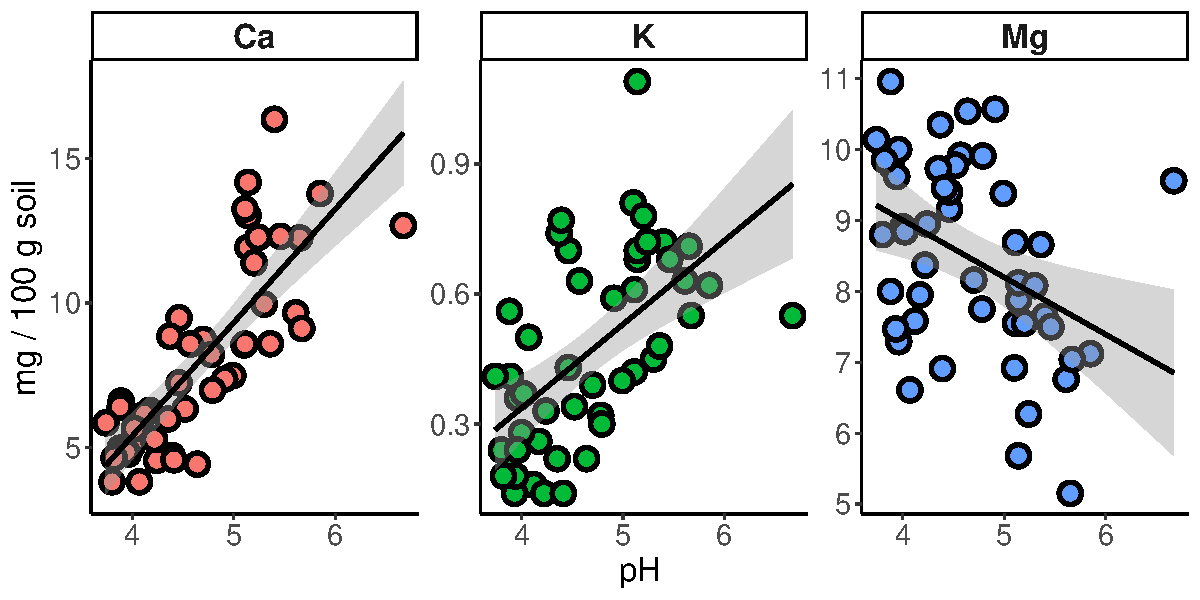
\includegraphics{module1_3_files/figure-latex/unnamed-chunk-36-1.pdf}

\hypertarget{density-curves-and-error-bars}{%
\subsubsection{Density curves and error
bars}\label{density-curves-and-error-bars}}

Using \textbf{\texttt{geom\_smooth}} to plot trendlines is a useful way
to get more information from your scatterplots. To get an idea for how
other kinds of statistical elements can be drawn onto plots, we'll look
at examples using histograms and boxplots.

First, a simple histogram of 3 soil nutrients.

\begin{Shaded}
\begin{Highlighting}[]
\CommentTok{\# Adding density/smooth curves to plots}

   \DocumentationTok{\#\# first produce some histograms}

\FunctionTok{ggplot}\NormalTok{(soil.nut) }\SpecialCharTok{+}
  \FunctionTok{geom\_histogram}\NormalTok{(}\FunctionTok{aes}\NormalTok{(}\AttributeTok{x=}\NormalTok{value), }\AttributeTok{color=}\StringTok{"black"}\NormalTok{, }\AttributeTok{fill=}\StringTok{"white"}\NormalTok{, }\AttributeTok{bins=}\DecValTok{15}\NormalTok{) }\SpecialCharTok{+}
  \FunctionTok{facet\_wrap}\NormalTok{(}\SpecialCharTok{\textasciitilde{}}\NormalTok{nutrient, }\AttributeTok{scales=}\StringTok{"free"}\NormalTok{) }\SpecialCharTok{+}
  \FunctionTok{xlab}\NormalTok{(}\StringTok{"mg / 100g soil"}\NormalTok{) }\SpecialCharTok{+}
  \FunctionTok{theme\_classic}\NormalTok{() }\SpecialCharTok{+}
  \FunctionTok{theme}\NormalTok{(}\AttributeTok{axis.text =} \FunctionTok{element\_text}\NormalTok{(}\AttributeTok{size=}\DecValTok{20}\NormalTok{),}
        \AttributeTok{axis.title =} \FunctionTok{element\_text}\NormalTok{(}\AttributeTok{size=}\DecValTok{25}\NormalTok{),}
        \AttributeTok{strip.text =} \FunctionTok{element\_text}\NormalTok{(}\AttributeTok{size=}\DecValTok{25}\NormalTok{, }\AttributeTok{face=}\StringTok{"bold"}\NormalTok{))}
\end{Highlighting}
\end{Shaded}

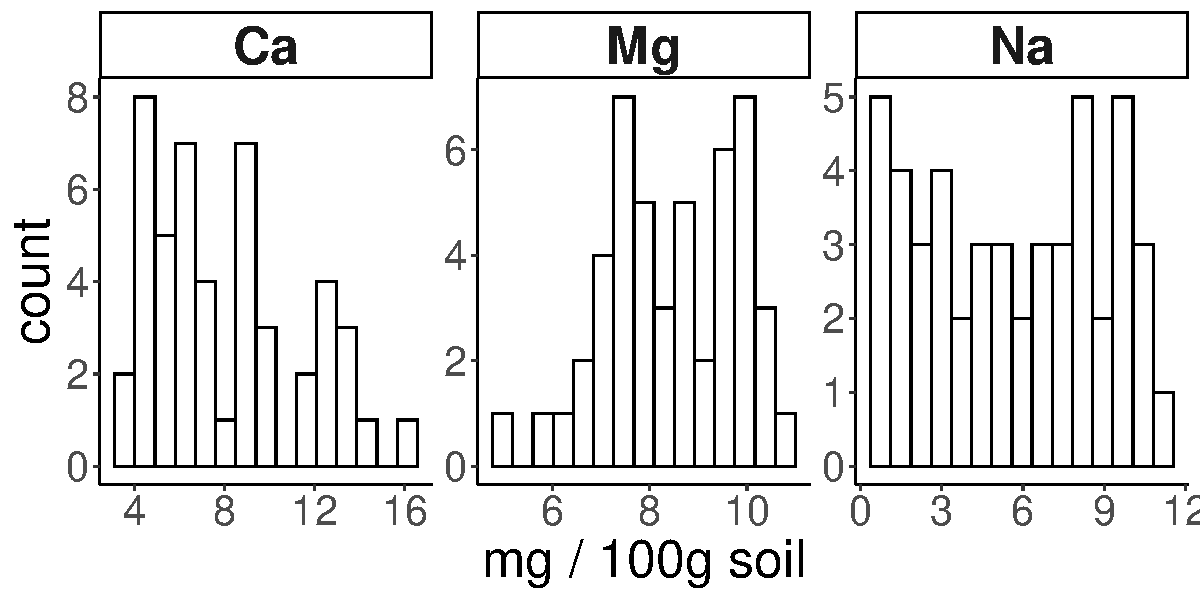
\includegraphics{module1_3_files/figure-latex/unnamed-chunk-37-1.pdf}

Here is how to add a density curve to the histogram with another
\textbf{\texttt{geom}}:

\begin{Shaded}
\begin{Highlighting}[]
\CommentTok{\# Then add density curves}

\FunctionTok{ggplot}\NormalTok{(soil.nut) }\SpecialCharTok{+}
  \FunctionTok{geom\_histogram}\NormalTok{(}\FunctionTok{aes}\NormalTok{(}\AttributeTok{x=}\NormalTok{value, }\AttributeTok{y=}\NormalTok{..density..), }\AttributeTok{color=}\StringTok{"black"}\NormalTok{, }\AttributeTok{fill=}\StringTok{"white"}\NormalTok{, }\AttributeTok{bins=}\DecValTok{15}\NormalTok{) }\SpecialCharTok{+}
  \FunctionTok{geom\_density}\NormalTok{(}\FunctionTok{aes}\NormalTok{(}\AttributeTok{x=}\NormalTok{value,}\AttributeTok{color=}\NormalTok{nutrient), }\AttributeTok{size=}\FloatTok{1.5}\NormalTok{) }\SpecialCharTok{+}
  \FunctionTok{facet\_wrap}\NormalTok{(}\SpecialCharTok{\textasciitilde{}}\NormalTok{nutrient, }\AttributeTok{scales=}\StringTok{"free"}\NormalTok{) }\SpecialCharTok{+}
  \FunctionTok{xlab}\NormalTok{(}\StringTok{"mg / 100g soil"}\NormalTok{) }\SpecialCharTok{+}
  \FunctionTok{theme\_classic}\NormalTok{() }\SpecialCharTok{+}
  \FunctionTok{theme}\NormalTok{(}\AttributeTok{legend.position=}\StringTok{"none"}\NormalTok{,}
        \AttributeTok{axis.text =} \FunctionTok{element\_text}\NormalTok{(}\AttributeTok{size=}\DecValTok{20}\NormalTok{),}
        \AttributeTok{axis.title =} \FunctionTok{element\_text}\NormalTok{(}\AttributeTok{size=}\DecValTok{25}\NormalTok{),}
        \AttributeTok{strip.text =} \FunctionTok{element\_text}\NormalTok{(}\AttributeTok{size=}\DecValTok{25}\NormalTok{, }\AttributeTok{face=}\StringTok{"bold"}\NormalTok{))}
\end{Highlighting}
\end{Shaded}

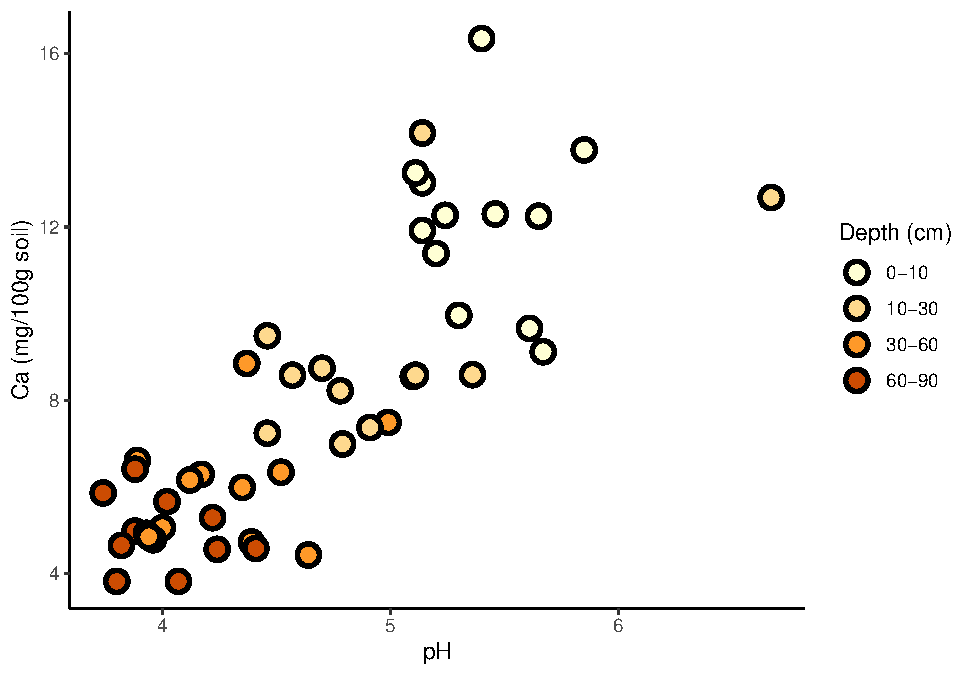
\includegraphics{module1_3_files/figure-latex/unnamed-chunk-38-1.pdf}

And here's how we can compare our distributions to a normal
distribution, using a \textbf{\texttt{stat}} function:

\begin{Shaded}
\begin{Highlighting}[]
\CommentTok{\# And now let\textquotesingle{}s use a statistical function (dnorm) in ggplot to compare with a normal distribution:}

\FunctionTok{ggplot}\NormalTok{(soil.nut) }\SpecialCharTok{+}
  \FunctionTok{geom\_histogram}\NormalTok{(}\FunctionTok{aes}\NormalTok{(}\AttributeTok{x=}\NormalTok{value, }\AttributeTok{y=}\NormalTok{..density..), }\AttributeTok{color=}\StringTok{"black"}\NormalTok{, }\AttributeTok{fill=}\StringTok{"white"}\NormalTok{, }\AttributeTok{bins=}\DecValTok{15}\NormalTok{) }\SpecialCharTok{+}
  \FunctionTok{stat\_function}\NormalTok{(}\AttributeTok{fun =}\NormalTok{ dnorm, }\AttributeTok{color =} \StringTok{"blue"}\NormalTok{, }\AttributeTok{size =} \FloatTok{1.5}\NormalTok{,}
                \AttributeTok{args=}\FunctionTok{list}\NormalTok{(}\AttributeTok{mean=}\FunctionTok{mean}\NormalTok{(soil.nut}\SpecialCharTok{$}\NormalTok{value), }\AttributeTok{sd=}\FunctionTok{sd}\NormalTok{(soil.nut}\SpecialCharTok{$}\NormalTok{value))) }\SpecialCharTok{+}
  \FunctionTok{facet\_wrap}\NormalTok{(}\SpecialCharTok{\textasciitilde{}}\NormalTok{nutrient, }\AttributeTok{scales=}\StringTok{"free"}\NormalTok{) }\SpecialCharTok{+}
  \FunctionTok{xlab}\NormalTok{(}\StringTok{"mg / 100g soil"}\NormalTok{) }\SpecialCharTok{+}
  \FunctionTok{theme\_classic}\NormalTok{() }\SpecialCharTok{+}
  \FunctionTok{theme}\NormalTok{(}\AttributeTok{legend.position=}\StringTok{"none"}\NormalTok{,}
        \AttributeTok{axis.text =} \FunctionTok{element\_text}\NormalTok{(}\AttributeTok{size=}\DecValTok{20}\NormalTok{),}
        \AttributeTok{axis.title =} \FunctionTok{element\_text}\NormalTok{(}\AttributeTok{size=}\DecValTok{25}\NormalTok{),}
        \AttributeTok{strip.text =} \FunctionTok{element\_text}\NormalTok{(}\AttributeTok{size=}\DecValTok{25}\NormalTok{, }\AttributeTok{face=}\StringTok{"bold"}\NormalTok{))}
\end{Highlighting}
\end{Shaded}

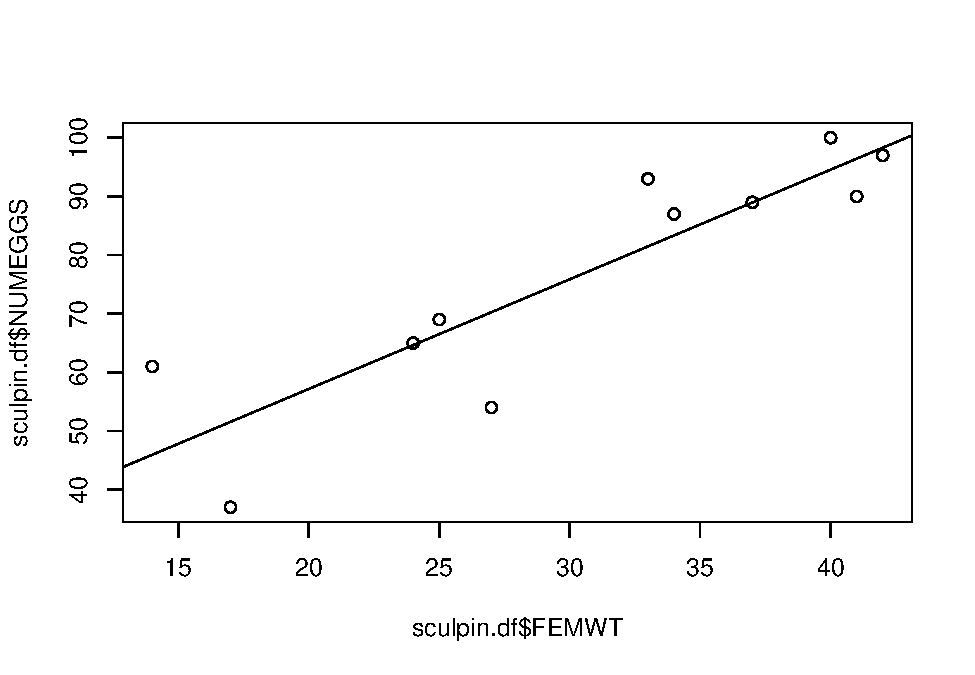
\includegraphics{module1_3_files/figure-latex/unnamed-chunk-39-1.pdf}

Let's go back to our basic boxplot, the default plot for visualizing
continuous data against categories.

First, you may have noticed that the whiskers do not have caps on them,
as they do in base R. This is a matter of personal preference, but if
capless whiskers look ``off'' to you, then you can work around it using
\textbf{\texttt{stat\_boxplot}}. \textbf{\texttt{stat\_}} functions are
another group of functions for creating layers based on statistical
properties of the data. Another example is
\textbf{\texttt{stat\_summary}}, which we use in the example below to
add means to the boxplot.

\begin{Shaded}
\begin{Highlighting}[]
\CommentTok{\# add error bars and other stat summaries (e.g., mean) to boxplot}

\FunctionTok{ggplot}\NormalTok{(soil, }\FunctionTok{aes}\NormalTok{(}\AttributeTok{x=}\NormalTok{Contour, }\AttributeTok{y=}\NormalTok{pH)) }\SpecialCharTok{+}
  \FunctionTok{stat\_boxplot}\NormalTok{(}\AttributeTok{geom=}\StringTok{"errorbar"}\NormalTok{, }\AttributeTok{width=}\FloatTok{0.2}\NormalTok{) }\SpecialCharTok{+}  
  \FunctionTok{stat\_boxplot}\NormalTok{() }\SpecialCharTok{+}
  \FunctionTok{stat\_summary}\NormalTok{(}\AttributeTok{fun=}\NormalTok{mean,}\AttributeTok{geom=}\StringTok{"point"}\NormalTok{,}\AttributeTok{size=}\DecValTok{5}\NormalTok{, }\AttributeTok{color=}\StringTok{"black"}\NormalTok{)}
\end{Highlighting}
\end{Shaded}

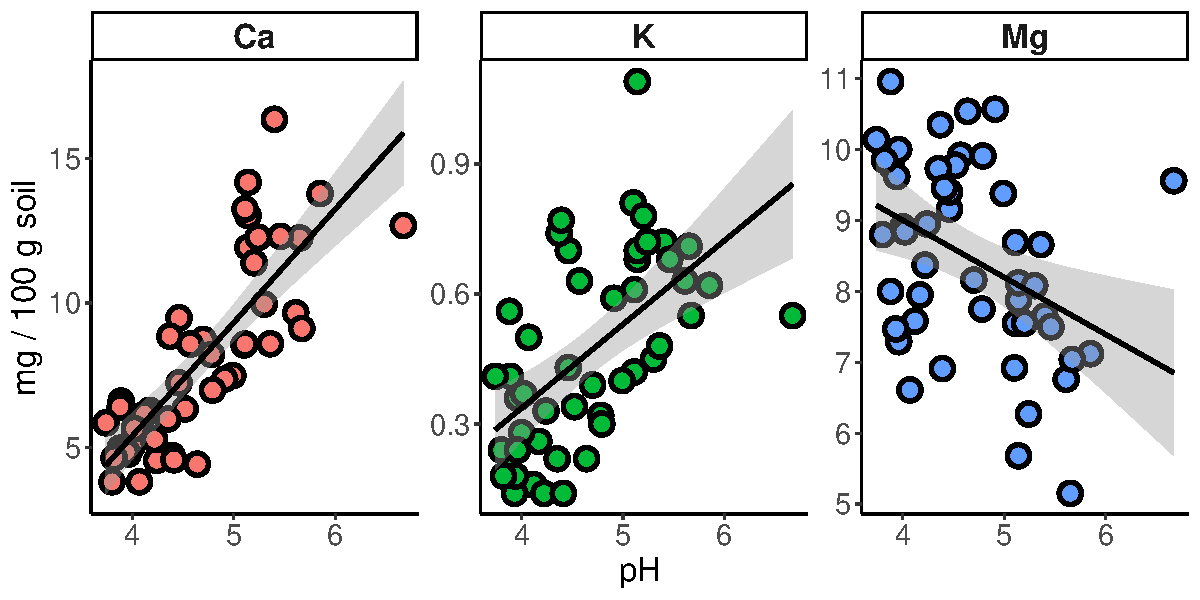
\includegraphics{module1_3_files/figure-latex/unnamed-chunk-40-1.pdf}

Interestingly, there is generally a way to add just about any graphical
element using either ``stat\_'' or ``geom\_'' functions. It's a good
idea to play around with both!

\hypertarget{technique-specific-plotting-libraries}{%
\subsubsection{Technique-specific plotting
libraries}\label{technique-specific-plotting-libraries}}

Several analytical packages come with their own plotting functions that
produce some very nice visualizations. There are dozens out there, but a
few of them are
\href{https://cran.r-project.org/web/packages/visreg/visreg.pdf}{visreg}
for regression plots,
\href{https://cran.r-project.org/web/packages/corrplot/index.html}{corrplot}
(and its ggplot counterpart,
\href{http://www.sthda.com/english/wiki/ggcorrplot-visualization-of-a-correlation-matrix-using-ggplot2}{ggcorrplot})
for graphical presentation of correlation matrices, and
\href{https://cran.r-project.org/web/packages/rpart.plot/index.html}{rpart.plot}
as a companion to the decision tree package rpart.

\end{document}
